\documentclass[aps,floatfix,10pt,amssymb,amsfont,amsmath,superscriptaddress,float,nofootinbib,longbibliography,nobalancelastpage,twocolumn]{revtex4-2}
\usepackage{graphicx} % Required for inserting images
\usepackage{hyperref}
\hypersetup{hidelinks}
\usepackage{braket}
\usepackage{amsfonts}
\usepackage{amssymb}
\usepackage{amsmath}
\usepackage{bbm}
\usepackage{bm}
\usepackage[english]{babel}
\usepackage{amsthm}
\newtheorem{theorem}{Theorem}
\newtheorem{lemma}{Lemma}
\newtheorem{duplicate}{Theorem}
\newtheorem{corollary}{Corollary}
\newtheorem{remark}{Remark}
\usepackage{subfig}
\usepackage{tikz}
\usetikzlibrary{arrows,positioning}
 \usetikzlibrary{quotes}
\usepackage{yquant}
\pgfdeclareshape{yquant-multictrlshape}{
   \inheritsavedanchors[from=yquant-circle]%
   \foreach \anc in {center, north, north east, east, south east, south, south west, west, north west} {%
      \inheritanchor[from=yquant-circle]{\anc}%
   }%
   \inheritanchorborder[from=yquant-circle]%
   \backgroundpath{%
      \pgfpathmoveto{\pgfqpoint{-0.707107\dimexpr\xradius\relax}{-0.707107\dimexpr\yradius\relax}}%
      \pgfpathlineto{\pgfqpoint{0.707107\dimexpr\xradius\relax}{0.707107\dimexpr\yradius\relax}}%
      \pgfpathellipse{\pgfpointorigin}%
                     {\pgfqpoint{\xradius}{0pt}}%
                     {\pgfqpoint{0pt}{\yradius}}%
   }%
   \inheritclippath[from=yquant-circle]%
}

\yquantset{multictrl/.style={every negative control/.style={draw, /yquant/default fill,shape=yquant-multictrlshape,radius=1.05mm}}}
\pgfdeclareshape{yquant-bctrlshape}{
   \inheritsavedanchors[from=yquant-circle]%
   \foreach \anc in {center, north, north east, east, south east, south, south west, west, north west} {%
      \inheritanchor[from=yquant-circle]{\anc}%
   }%
   \inheritanchorborder[from=yquant-circle]%
   \backgroundpath{%
      % Draw the circle
      \pgfpathellipse{\pgfpointorigin}%
                     {\pgfqpoint{\xradius}{0pt}}%
                     {\pgfqpoint{0pt}{\yradius}}%
   }%
   % Add the "b" in the center
   \foregroundpath{%
      \pgftext[center]{\(\scriptstyle b\)}%
   }%
   \inheritclippath[from=yquant-circle]%
}

\yquantset{
  bctrl/.style={
    every control/.style={
      draw,
      /yquant/default fill,
      shape=yquant-bctrlshape,
      radius=1.05mm
    }
  }
}
\date{February 2025}
\begin{document}
\yquantdefinebox{dots}[inner sep=0pt]{$\dots$}

\title{New and Improved Quantum Metropolis Sampling}
\author{Oliver O'Brien}
\affiliation{Department of Applied Mathematics and Theoretical Physics, University of Cambridge,\\ Wilberforce Road, Cambridge, CB3 0WA, United Kingdom}
\author{Rakesh Achutha}
\affiliation{Department of Applied Mathematics and Theoretical Physics, University of Cambridge,\\ Wilberforce Road, Cambridge, CB3 0WA, United Kingdom}
\author{Frank Verstraete}
\affiliation{Department of Applied Mathematics and Theoretical Physics, University of Cambridge,\\ Wilberforce Road, Cambridge, CB3 0WA, United Kingdom}
\affiliation{Department of Physics and Astronomy, Ghent University, Krijgslaan 281, 9000 Gent, Belgium}

\begin{abstract}
    We introduce a resource-efficient protocol for Boosted State-Independent Quantum Phase Estimation (BSI-QPE), enabling practical implementation of the Quantum Metropolis algorithm. By employing window functions to suppress fat tails, our approach maintains coherence and shift invariance required for reversible sampling. We reframe the rejection process using a two-dimensional invariant subspace. A modified formulation of approximate quantum detailed balance is proposed, ensuring convergence to Gibbs states under realistic error bounds. These advancements significantly lower the resource threshold for quantum thermal state preparation.
\end{abstract}

\maketitle

\section{Introduction}
The Quantum Metropolis algorithm, first proposed by Temme et al. \cite{Temme_2011}, remains one of the most promising quantum algorithms for sampling from Gibbs (thermal) states of quantum systems. These states are fundamental in statistical mechanics and appear across condensed matter physics, quantum chemistry, and high-energy physics, where accurate thermal state preparation is a central computational challenge. 

However, the algorithm as originally stated suffers from two major issues which have led the community to investigate alternative gibbs sampling techniques (\cite{}). Firstly, \cite{Temme_2011} heavily relies upon phase estimation and hence has to deal with the resultant fat tails \cite{}.  Numerous solutions to this problem have been explored (\cite{}). In the original paper \cite{Temme_2011} it was posited that coherently taking the median of multiple phase estimations could help boost the signal and remove these fat tails. However, the phase estimation is also required to be shift invariant which the median trick struggles to fulfill. Recently, \cite{chen2023quantumthermalstatepreparation} proved a no-go theorem suggesting that it is not possible to implement the boosted shift-invariant phase estimation required by the quantum metropolis algorithm. 

We propose a boosted shift-invariant phase estimation protocol which utilises window functions to exponentially dampen the fat tails. This drastically reduces the number of ancilla qubits required for the algorithm to work, and also conclusively proves that quantum metropolis does indeed work. 

In Section \ref{section:boostedphaseestimation} we present the construction of the Boosted Shift-Invariant Quantum Phase Estimation (BSI-QPE) protocol, including a detailed circuit-level description and error analysis based on window functions. In Section \ref{section:algorithm}, we describe our modified Quantum Metropolis algorithm incorporating our improved quantum phase estimation. This includes a novel understanding of the rewinding mechanism formulated through iterative projective measurements and invariant subspaces. Section \ref{section:why} rigorously proves that our algorithm satisfies an approximate quantum detailed balance condition and discusses the convergence guarantees to the thermal Gibbs state. Finally, in Section \ref{section:discussion}, we discuss the broader implications of our results, the assumptions made, and the outlook for implementing these techniques on near-term or fault-tolerant quantum hardware.


\section{Boosted State-Independent Quantum Phase Estimation}
\label{section:boostedphaseestimation}
Given an $m$-qubit Hamiltonian $H$ with eigenvectors $\ket{\psi_j}$ such that $H\ket{\psi_j} = E_j \ket{\psi_j}$, quantum phase estimation (QPE) allows one to prepare an ancilla register that approximates $E_j$. Unfortunately, quantum computers have limited precision. As a result, unless the energy can be represented exactly in binary using $\eta$ bits (corresponding to $\eta$ ancilla qubits), there is a high probability of obtaining an inaccurate energy measurement. This inaccuracy arises from the ``fat tails" in QPE \cite{Nielsen_Chuang_2010}.

Often this issue can be mitigated by simply repeating the calculation and taking an average. However, quantum metropolis sampling requires us to ``rewind" upon rejecting a proposed update and hence we require a unitary method for ``boosting" QPE. This ``boosted" QPE stores an approximation to the energy in ancillas which is not immediately measured but rather used as the basis for further coherent calculations. Further, for ``rewinding" to work we must reuse the same ancilla registers so the QPE protocol must also be state-independent. Therefore, we must demonstrate an implementation of a boosted state-independent quantum phase estimation (BSI-QPE). While it has been shown \cite{chen2023quantumthermalstatepreparation} that QPE cannot entirely eliminate the probability mass in its tails, we demonstrate that it is possible to construct BSI-QPE protocols with exponentially suppressed tails, which effectively mitigate the issue for practical purposes. 

Existing methods for boosting QPE rely upon choosing specific input ancillary states. In these methods QPE is performed using ancillas initialised to the state $\sum_x \alpha(x) \ket{x}$ for some window function $\alpha(x)$ instead of the standard uniform superposition. After performing QPE upon eigenstate $\ket{\psi_j}$ the following state is produced:
\begin{equation}
   \frac{1}{\sqrt{2^{\eta}}} \sum_x \sum_k e^{\frac{2 \pi i}{2^{\eta}}x(k-E_j)} \alpha(x)\ket{k}\ket{\psi_j}
\end{equation}
which can be rewritten as:
\begin{equation}
    \sum_k \hat\alpha(k-E_j) \ket{k}\ket{\psi_j}
\end{equation}
where $\hat \alpha(k)$ is the discrete Fourier transform of $\alpha(x)$. By choosing $\alpha$ to be a window function one can ensure that $\hat \alpha$ is narrowly peaked, thus QPE is boosted. Unfortunately, this is not sufficient for the quantum Metropolis algorithm as we require the QPE to be independent of the ancillary state, as we must reuse the same ancillas throughout the rewinding process. 

Our construction uses two window functions $\alpha(x)$ and $\beta(x) = \sqrt{1-\alpha(x)^2}$ (for $x\in\{0,1,\ldots,2^{\eta}-1\}$) which are both narrowly peaked in the Fourier domain. We introduce these windows via the following multi-controlled single-qubit rotation:
\begin{equation}
   CR_Y = \sum_k \ket{k}\bra{k}\otimes \begin{pmatrix}
        \alpha(k)& \beta(k)\\
        -\beta(k)& \alpha(k)
    \end{pmatrix}
\end{equation}

We also require the following time evolution gadget which is constructed as shown in Fig~\ref{fig:CRZ}:
\begin{equation}
    CR_Z =\sum_{j,k}\ket{\psi_j}\bra{\psi_j}\otimes\ket{k}\bra{k} \otimes \begin{pmatrix}
        e^{\frac{iE_jkt}{2}}&0\\
        0 & e^{-\frac{iE_jkt}{2}}
    \end{pmatrix}
\end{equation}
\begin{figure*}
\[
\vcenter{\hbox{
\resizebox{!}{2.5cm}{
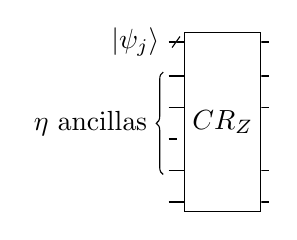
\begin{tikzpicture}
\begin{yquant*}
qubit {$\ket{\psi_j}$} s;

init {$\eta$ ancillas} (a[0,1],ellipsis, aend);
slash s;
hspace {0.1cm} -;
discard ellipsis;
% qubit {} aend;
qubit {} f;
box {$CR_Z$} (s,a,ellipsis, aend, f);

% text {$\ket{0}$} f;
\end{yquant*}
\end{tikzpicture}}}}
=
\vcenter{\hbox{
\resizebox{!}{2.5cm}{
    \begin{tikzpicture}
\begin{yquant*}
qubit {$\ket{\psi_j}$} s;

init {$\eta$ ancillas} (a[0,1],ellipsis, aend);
discard ellipsis;
% qubit {} aend;
qubit {} f;
slash s;
hspace {0.1cm} -;

box {$U^{\dagger 2^0}$} (s) | a[0], f;
box {$U^{\dagger 2^1}$} (s) | a[1], f;
hspace {0mm} -;
dots ellipsis;

box {$U^{\dagger 2^{\eta-1}}$} (s) | aend[0], f;
box {$U^{2^0}$} (s) | a[0]~ f;
box {$U^{ 2^1}$} (s) | a[1]~ f;
hspace {0mm} -;
dots ellipsis;

box {$U^{ 2^{\eta-1}}$} (s) | aend[0]~ f;
\end{yquant*}
\end{tikzpicture}}}}
\]
\caption{Quantum circuit for implementing an $Z$ rotation on an ancilla qubit that is dependent upon the energy of the system. The unitary $U=e^{\frac{iHt}{2}}$ is implemented through some quantum time evolution algorithm (e.g. trotterisation \cite{lloyd1996universal}, qubitization \cite{Low2019hamiltonian}) up to an operator norm error of $\epsilon^T_t$. Throughout this work we assume  $\epsilon^T_t$ is negligible, and use perfect quantum time evolution in our error analysis.}
    \label{fig:CRZ}
\end{figure*}
Both of these act as controlled $R_Z$ and $R_Y$ rotations on a single qubit. 
\begin{figure*}
\[
\vcenter{\hbox{
\resizebox{!}{2.5cm}{
\begin{tikzpicture}
    \begin{yquant*}
qubit {$\ket{\psi_j}$} s;

init {$\eta$ ancillas} (a[0,1],ellipsis, aend);
slash s;
% hspace {0.1cm} -;
discard ellipsis;
% qubit {} aend;
qubit {} f;
dots ellipsis;

box {BSI-\\QPE} (s,a,ellipsis, aend, f);

% text {$\ket{0}$} f;
\end{yquant*}
\end{tikzpicture} }}}
=
\vcenter{\hbox{
\resizebox{!}{2.5cm}{
\begin{tikzpicture}
    \begin{yquant*}
qubit {$\ket{\psi_j}$} s;

init {$\eta$ ancillas} (a[0,1],ellipsis, aend);
slash s;
discard ellipsis;
% qubit {} aend;
qubit {} f;
dots ellipsis;
box {QFT} (a,ellipsis, aend);

[this subcircuit box style={dashed, "$R_Z[E_jt(k-k')]$"}]
subcircuit {
qubit {} s;
qubit {} a[2];
nobit ellipsis;
qubit {} aend;
qubit {} f;

% dots ellipsis;
box {$CR_Z$} (s,a,ellipsis, aend, f);

x aend[0];
dots ellipsis;
box {$CR_Z^{\dagger}$} (s,a,ellipsis, aend, f);
x aend[0];
dots ellipsis;
} (s,a,ellipsis, aend, f);

box {$CR_Y$} (a,ellipsis, aend, f);

[this subcircuit box style={dashed, "$R_Z[E_jt(k+k'-2^{\eta})]$"}]
subcircuit {
qubit {} s;
qubit {} a[2];
nobit ellipsis;
qubit {} aend;
qubit {} f;

box {$CR_Z$} (s,a,ellipsis, aend, f);
x aend[0];
dots ellipsis;
box {$CR_Z$} (s,a,ellipsis, aend, f);
x aend[0];
dots ellipsis;
box {$U^{\dagger 2^{\eta}}$} (s) ~ f;
box {$U^{2^{\eta}}$} (s) | f;
} (s,a,ellipsis, aend, f);

box {iQFT} (a,ellipsis, aend);

% text {$\ket{0}$} f;
\end{yquant*}
\end{tikzpicture} }}}
\]

\caption{Quantum circuit implementing boosted state-independent quantum phase estimation (BSI-QPE). We highlight how the combinations of $CR_Z$ and $X$ gates operators correspond to the single qubit $R_Z$ given in Eq.~\ref{eq:euler} with $k$ being the value stored in the $\eta$ ancillas and $k' = k + 2^{\eta-1} \mod 2^{\eta}$}
\label{fig:circuit}
\end{figure*}
\begin{figure*}
\begin{tikzpicture}
    \begin{yquant*}
qubit {$\ket{\psi_j}$} s;

init {$\eta$ ancillas} (a[0,1],ellipsis, aend);
slash s;
discard ellipsis;
% qubit {} aend;
dots ellipsis;
box {QFT} (a,ellipsis, aend);

box {$U^{ 2^1}$} (s) | a[0];
box {$U^{ 2^2}$} (s) | a[1];
hspace {0mm} -;
dots ellipsis;

box {$U^{ 2^{\eta}}$} (s) | aend[0];
box {$U^{\dagger 2^{\eta}}$} (s);
box {iQFT} (a,ellipsis, aend);

% text {$\ket{0}$} f;
\end{yquant*}
\end{tikzpicture} 

\caption{Quantum circuit implementing unboosted state-independent QPE with $U=e^{\frac{iHt}{2}}$, equivalent to choosing $\alpha(x)=1$ for BSI-QPE and acting upon $\ket{0}_F$. This slightly differs from the standard formulation of QPE \cite{Nielsen_Chuang_2010} by beginning with $QFT$ rather than $H^{\otimes \eta}$ and the addition of $U^{\dagger 2^{\eta}}$ at the end. }
\label{fig:standard_qpe}
\end{figure*}

\begin{widetext}
We can implement BSI-QPE through the circuit illustrated in Fig~\ref{fig:circuit}. This circuit combines the  $CR_Z$ and $CR_Y$ rotations using the following $R_ZR_YR_Z$ decomposition \cite{Nielsen_Chuang_2010}: 
\begin{equation}
\label{eq:euler}
    R_Z[E_jt(k+k'-2^{\eta})]R_Y[2\arccos(\alpha(k))]R_Z[E_jt(k-k')] = \begin{pmatrix}
        \alpha(k)e^{iE_jtk}e^{-iE_jt2^{\eta-1}} && \beta(k)e^{iE_jt k'}e^{-iE_jt2^{\eta-1}}\\
        -\beta (k)e^{-iE_jt k'}e^{iE_jt2^{\eta-1}} && \alpha(k)e^{-iE_jtk}e^{iE_jt2^{\eta-1}}
    \end{pmatrix}
\end{equation}
In Fig.~\ref{fig:circuit}, the $X$-gates acting on the last qubit in the ancilla register shift the value stored from $k$ to $k'= k+2^{\eta-1} \mod 2^{\eta}$, and hence we get the following operation:
\begin{multline}
        \text{BSI-QPE} = \frac{1}{2^{\eta}}\sum_j\sum_{p,q,k} \begin{pmatrix}
        \alpha(k)e^{iE_jtk}e^{-iE_jt2^{\eta-1}} && \beta(k)e^{iE_jt[(k+2^{\eta-1})\text{mod} 2^{\eta}]}e^{-iE_jt2^{\eta-1}}\\
        -\beta (k)e^{-iE_jt[(k+2^{\eta-1})\text{mod} 2^{\eta}]}e^{iE_jt2^{\eta-1}} && \alpha(k)e^{-iE_jtk}e^{iE_jt2^{\eta-1}}
    \end{pmatrix}e^{\frac{2\pi i}{2^{\eta}}k(q-p)} \\\otimes\ket{p}\bra{q}\otimes\ket{\psi_j}\bra{\psi_j}
\end{multline}
Throughout the remainder of this work we write
\begin{equation}
    \omega_j = \frac{2^{\eta}t}{2\pi}E_j
    \label{eq:omegadef}
\end{equation}
for the eigenenergy $E_j$ expressed in units of phase-estimation bins. The operator above can then be simplified to:
\begin{equation}
    \text{BSI-QPE} = \frac{1}{\sqrt{2^{\eta}}}\sum_j\sum_{p,q} \begin{pmatrix}
        (-1)^{q-p}\hat\alpha(q-p+\omega_{j}) && \hat\beta(q-p+\omega_{j})\\
        -\hat\beta (q-p-\omega_{j}) && (-1)^{q-p}\hat\alpha(q-p-\omega_{j})
    \end{pmatrix}\otimes\ket{p}\bra{q}\otimes\ket{\psi_j}\bra{\psi_j}
\end{equation}
% \begin{multline}
%   \sum_j \sum^{2^{\eta}}_{p,q} \hat \alpha(p - q - \frac{2^{\eta} t}{2\pi}E_j)\ket{0}\bra{0} \otimes\ket{p}\bra{q} \otimes \ket{\psi_j} \bra{\psi_j}\\
%   + \ket{0}\bra{0} \otimes\bm{\varepsilon}^T_{kt}
% \end{multline}
where $\hat \alpha$ is the discrete Fourier transform of $\alpha$ as given by:
\begin{equation}
   \hat\alpha(x) =\frac{1}{\sqrt{2^{\eta}}}\sum_{k=-2^{\eta-1}}^{2^{\eta-1}-1} \alpha(k+2^{\eta-1})e^{\frac{2\pi i}{2^{\eta}}xk}
\end{equation}
and $\hat \beta$ is the discrete Fourier transform of $\beta$ given by:
\begin{equation}
    \hat\beta(x) =\frac{1}{\sqrt{2^{\eta}}}\sum_{k=-2^{\eta-1}}^{2^{\eta-1}-1} \beta(k)e^{\frac{2\pi i}{2^{\eta}}kx}
\end{equation}
 where $\beta(k)$ is extended by $\beta(k) = \beta(k \mod 2^{\eta})$. We have defined $\hat \alpha$ as the discrete Fourier transform of $\alpha(k)$ shifted by $2^{\eta-1}$. This is essential as $|\alpha|^2+|\beta|^2=1$, so without this shift we cannot have both $\alpha, \beta \ll1$ at the boundary of the discrete Fourier transform and hence we would observe spectral leakage (for non-integer $k$) that precludes exponentially decaying tails. Throughout the rest of this work, we will use the following notational shorthand: 
\begin{equation}
\label{eq:G}
    G_j^{pq} = \begin{pmatrix}
        (-1)^{q-p}\hat\alpha(q-p+\omega_{j}) && \hat\beta(q-p+\omega_{j})\\
        -\hat\beta (q-p-\omega_{j}) && (-1)^{q-p}\hat\alpha(q-p-\omega_{j})
    \end{pmatrix}
\end{equation}
It is worth pausing on the physical content of $G^{pq}_j$: BSI-QPE shifts the energy-index register by approximately $\pm\omega_j$, in a direction set by the qubit $F$. The $\hat\alpha$ entries implement the shift $q \approx p \mp \omega_j$ without flipping $F$, while the $\hat\beta$ entries implement the same shifts accompanied by an $F$ flip; in all four entries the amplitude is concentrated in a window of width $\sim\mu$ around the ideal shift (Fig.~\ref{fig:windowcartoon}). It is this concentration that later ties every measurement record to the energies of the states involved.
\end{widetext}
There are many potential candidates for window functions $\alpha(x)$ and $\beta(x)$. In this work we choose to work with $\alpha(x) = \text{sech}( r\cos^{2b} \frac{\pi x}{2^{\eta}})$ and $\beta(x) = \text{tanh}(r \cos^{2b} \frac{\pi x}{2^{\eta}})$. These can both be shown to have discrete Fourier transforms which decay exponentially fast as we discuss in Appendix~\ref{section:appendix}:
\begin{equation}
    |\hat \alpha(k)|,|\hat \beta(k)| = O\left( \sqrt{2^{\eta}}e^{-\nu |k|}\right)
    \label{eq:scaling}
\end{equation}
where $\nu = \frac{1}{3}\sin^2\frac{\pi}{4b}$. Equation~\eqref{eq:scaling} holds under the parameter conditions collected in the summary box at the end of Appendix~\ref{section:appendix} (in particular $A_0>\frac{1}{\sqrt{2}}$, i.e.\ $b > 1+\log_2\frac{r}{\pi}$, with $r$ chosen as prescribed there); we assume these conditions throughout. Hence we can write:
\begin{equation}
    \hat\alpha(k) = \tilde\alpha(k) + \Delta_{\alpha}(k) \>\>\>\>\>\>\hat\beta(k) = \tilde\beta(k) + \Delta_{\beta}(k)
    \label{eq:decomposealpha}
\end{equation}
where:
\begin{align}
    \tilde\alpha(k) &= \hat\alpha(k)\mathbbm{1}(|k|_{2^{\eta}}\leq \mu)\\
    \tilde\beta(k) &= \hat\beta(k)\mathbbm{1}(|k|_{2^{\eta}}\leq \mu)
    \label{eq:decomposealpha2}
\end{align}  and
\begin{equation}
    \sum_k|\Delta_\alpha(k)|,\sum_k|\Delta_\beta(k)|\leq \epsilon_{\Delta}
    \label{eq:decomposealpha3}
\end{equation} where $\epsilon_{\Delta} = O(\sqrt{2^{\eta}}e^{-\nu \mu})$ and $|x|_N = \min(x \mod N,- x\mod N)$ is the modular norm value of $x$.

\begin{figure}
    \centering
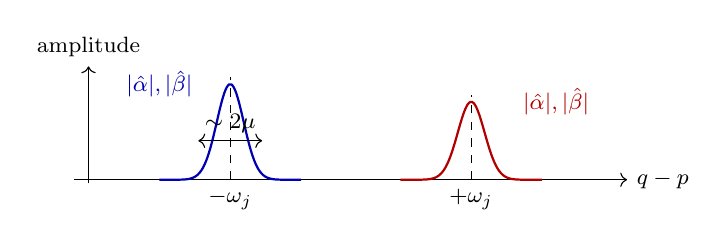
\begin{tikzpicture}[scale=0.9]
    \draw[->] (-0.2,0) -- (7.6,0) node[right] {\footnotesize $q-p$};
    \draw[->] (0,-0.05) -- (0,1.6) node[above] {\footnotesize amplitude};
    \draw[thick, blue!70!black, domain=1.0:3.0, samples=60, smooth] plot (\x, {1.35*exp(-14*(\x-2)*(\x-2))});
    \draw[thick, red!70!black, domain=4.4:6.4, samples=60, smooth] plot (\x, {1.1*exp(-14*(\x-5.4)*(\x-5.4))});
    \draw[dashed] (2,0) -- (2,1.45); \node[below] at (2,0) {\footnotesize $-\omega_j$};
    \draw[dashed] (5.4,0) -- (5.4,1.2); \node[below] at (5.4,0) {\footnotesize $+\omega_j$};
    \draw[<->] (1.55,0.55) -- (2.45,0.55); \node[above] at (2,0.52) {\footnotesize $\sim 2\mu$};
    \node[blue!70!black] at (1.0,1.35) {\footnotesize $|\hat\alpha|,|\hat\beta|$};
    \node[red!70!black] at (6.6,1.1) {\footnotesize $|\hat\alpha|,|\hat\beta|$};
\end{tikzpicture}
    \caption{Schematic of the two amplitude windows of $G^{pq}_j$ (Eq.~\ref{eq:G}). The register shift $q-p$ is concentrated within a bandwidth $\sim\mu$ of $\mp\omega_j$, with exponentially suppressed tails; which window is addressed is controlled by the qubit $F$.}
    \label{fig:windowcartoon}
\end{figure}
\begin{lemma}[Truncated BSI-QPE]
\label{lemma:0}
    Define $\widetilde{\text{BSI-QPE}}$ as given by:
    \begin{equation}
       \widetilde{\text{BSI-QPE}}= \frac{1}{\sqrt{2^{\eta}}}\sum_j \sum_{p,q} \tilde G^{pq}_j \otimes \ket{p}\bra{q} \otimes \ket{\psi_j}\bra{\psi_j}
    \end{equation}
    where 
    \begin{equation}
        \tilde G^{pq}_j = \begin{pmatrix}
        (-1)^{q-p}\tilde\alpha(q-p+\omega_{j}) && \tilde\beta(q-p+\omega_{j})\\
        -\tilde\beta (q-p-\omega_{j}) && (-1)^{q-p}\tilde\alpha(q-p-\omega_{j})
    \end{pmatrix}
    \end{equation}
    Then,  
    \begin{equation}
        \|\widetilde{\text{BSI-QPE}}-\text{BSI-QPE}\| \leq \frac{2\epsilon_{\Delta}}{\sqrt{2^{\eta}}}
    \end{equation}
\end{lemma}
The proof is a routine interpolation between the $\ell^1$ and $\ell^{\infty}$ norms of the truncated tails and is given in Appendix~\ref{app:perturbation}.
\begin{remark}[Why boosting is necessary]
Instead one could attempt to use unboosted state-independent QPE. This would correspond to choosing $\alpha(x)=1$, which simplifies Fig.~\ref{fig:circuit} to Fig.~\ref{fig:standard_qpe}. As this effectively acts as a rectangular window function, $|\hat\alpha(k)| = O(\frac{\sqrt{2^{\eta}}}{k})$ for off-grid $k$, so $\epsilon_{\Delta} = O(\sqrt{2^{\eta}}\log \frac{2^\eta}{\mu})$. This bound exceeds $\sqrt{2^{\eta}}$ and so unboosted state-independent QPE is insufficient for Quantum Metropolis sampling without the promise of energies exactly represented in $\eta$ bits.
\end{remark}
\section{Algorithm}
\label{section:algorithm}
Quantum metropolis is heavily inspired by the classical metropolis-hastings algorithm. The principal idea is to apply a randomly chosen update to the current state then accept/reject this update with a probability given by a function ($\tilde{f}_{E_aE_b}=\min(1, e^{-\beta(E_b-E_a)})$) of the energy before $(E_a)$ and after $(E_b)$ the update. This update process is repeated many times with the system quickly converging to equilibrium. To replicate this on a quantum computer we need to be able to: measure the energy of a state (Section~\ref{section:energymeasurement}), apply some update (Section~\ref{section:update}), accept/reject an update with the correct probability (Section~\ref{section:acceptprob}) and ``undo" an update upon deciding to reject it (Section~\ref{section:rejection}).
\paragraph*{Register conventions.}
Throughout one full update, let $R$ denote the $\eta$-qubit BSI-QPE energy-index register and qubit $F$ the additional qubit on which the $G_j^{pq}$ act. At the start of the update, $R$ is initialised to $\ket{0}$ whilst $F$ is in the maximally mixed state (by classically randomly choosing initial state $\ket{0}$ or $\ket{1}$) and the qubit $M$ on which the acceptance rotation $W_{abde}$ acts is initialized in $\ket{0}$. The same register $R$ and $F$ are used by $E_{ae}$ and by every subsequent $P_s^{ae}$ and $Q_s^{ae}$ measurement; it is never reset during the update. Likewise, $M$ is reused by every $Q_s^{ae}$ and is left untouched by $P_s^{ae}$. Fresh pointer qubits may be used to record measurement outcomes and are not part of the persistent work register.
\begin{figure}
    \centering
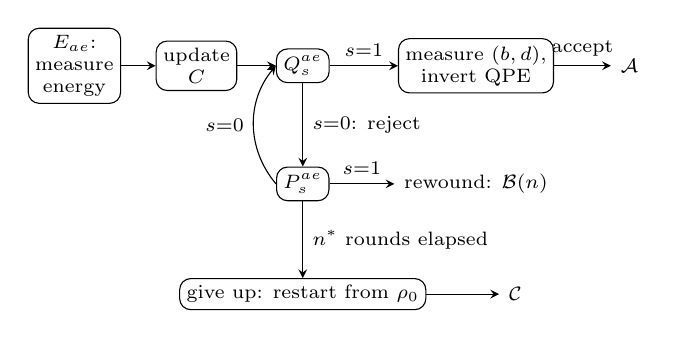
\begin{tikzpicture}[>=stealth, every node/.style={font=\scriptsize}]
    \tikzstyle{box}=[draw, rounded corners, inner sep=2.5pt, align=center]
    \node[box] (E) at (0,0) {$E_{ae}$:\\ measure\\ energy};
    \node[box] (C) at (1.55,0) {update\\ $C$};
    \node[box] (Q) at (2.9,0) {$Q^{ae}_s$};
    \node[box] (L) at (5.1,0) {measure $(b,d)$,\\ invert QPE};
    \node (acc) at (7.05,0) {$\mathcal{A}$};
    \node[box] (P) at (2.9,-1.5) {$P^{ae}_s$};
    \node (rej) at (5.1,-1.5) {rewound: $\mathcal{B}(n)$};
    \node[box] (F) at (2.9,-2.9) {give up: restart from $\rho_0$};
    \node (fail) at (5.6,-2.9) {$\mathcal{C}$};
    \draw[->] (E) -- (C);
    \draw[->] (C) -- (Q);
    \draw[->] (Q) -- node[above]{$s{=}1$} (L);
    \draw[->] (L) -- node[above]{accept} (acc);
    \draw[->] (Q) -- node[right]{$s{=}0$: reject} (P);
    \draw[->] (P) -- node[above]{$s{=}1$} (rej);
    \draw[->] (P.west) to[bend left=40] node[left]{$s{=}0$} (Q.west);
    \draw[->] (P) -- node[right]{$n^*$ rounds elapsed} (F);
    \draw[->] (F) -- (fail);
\end{tikzpicture}
    \caption{Anatomy of one update round. The first $Q^{ae}_s$ outcome decides acceptance; upon rejection the $P^{ae}_s/Q^{ae}_s$ loop attempts to rewind (outcomes of the in-loop $Q^{ae}_s$ are ignored), terminating when $P^{ae}_1$ signals a return to the initial energy record. The three terminal behaviours are the channels $\mathcal{A}$, $\mathcal{B}(n)$ and $\mathcal{C}$ of Section~\ref{section:why}. Fig.~\ref{fig:transitions} shows the induced Markov chain within one invariant subspace.}
    \label{fig:flowchart}
\end{figure}
\subsection{Measure the energy}
\label{section:energymeasurement}
To measure the energy we use the boosted state-independent quantum phase estimation protocol set out in Section~\ref{section:boostedphaseestimation}. We simply apply BSI-QPE, measure the ancilla qubits and then apply inverse BSI-QPE, as shown in Fig.~\ref{fig:Ecircuit} and outlined below:
\begin{multline}
    E_{ae} = \frac{1}{2^{\eta}}\sum_j\sum_{p_1,p_2,p_3,p_4} \ket{\psi_j}\bra{\psi_j} \otimes \ket{p_4}\braket{p_3|a}\braket{a|p_2}\bra{p_1} \otimes \\G_j^{p_3p_4 \dagger}\ket{e}\bra{e}G_j^{p_2p_1}
\end{multline}
\begin{multline}
        E_{ae} = \frac{1}{2^{\eta}}\sum_j\sum_{p_1,p_4} \ket{\psi_j}\bra{\psi_j}\otimes\ket{p_4}\bra{p_1}\otimes\\
        G_j^{ap_4 \dagger}\ket{e}\bra{e}G_j^{ap_1}
\end{multline}
\begin{figure}
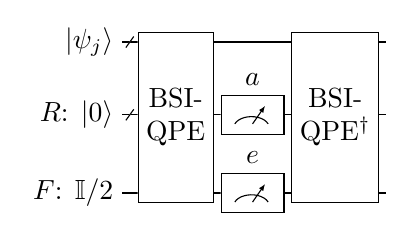
\begin{tikzpicture}
\begin{yquant*}
% init {$\eta$ ancillas} (a);
qubit {$\ket{\psi_j}$} system;
qubit {$R$: $\ket{0}$} a;
qubit {$F$: $\mathbb{I}/2$} f;

slash system;
slash a;
hspace {0.1cm} -;

box {BSI-\\QPE} (a,system,f);

["$a$",type=qubit]
measure a;

["$e$",type=qubit]
measure f;

box {BSI-\\QPE$^{\dagger}$} (a,system,f);
\end{yquant*}
\end{tikzpicture}

\caption{Quantum circuit for implementing projective measurement $E_{ae}$.}
\label{fig:Ecircuit}
\end{figure}
This measurement gives us $(-1)^ea$, which approximates the energy of the initial state. Because $E_{ae}$ is implemented as a projective measurement, its inverse BSI-QPE does not in general disentangle the work register. The post-measurement registers $R, F$ are retained and reused in all subsequent $P_s^{ae}$ and $Q_s^{ae}$ measurements in the same update.
\subsection{Update}
\label{section:update}
After measuring the initial energy we must apply an update to our state. In quantum metropolis this update comes in the form of a unitary operator $C$ chosen from some set $\mathcal{C}$ according to some probability measure $d\mu(C)$. It is essential for the purposes of detailed balance that the probability of choosing $C \in \mathcal{C}$ is equal to the probability of choosing $C^{\dagger} \in \mathcal{C}$ (which is alternatively expressed as $d\mu(C) = d\mu(C^{\dagger})$).
\subsection{Accept or Reject}
\label{section:acceptprob}
After applying our unitary update $C$ we must decide whether to accept or reject this update. To ensure the probability of acceptance is approximately $\tilde{f}_{E_aE_b}$, we use a combination of phase estimation, controlled rotations and single-qubit measurement (illustrated in Fig.~\ref{fig:Qcircuit}). First we apply phase estimation to the same registers $R, F$ used by $E_{ae}$. On the joint BSI-QPE space this operation is
\begin{equation}
   \frac{1}{\sqrt{2^{\eta}}}\sum_{j,b,p}G_j^{bp}\otimes\ket{b}\bra{p}\otimes\ket{\psi_j}\bra{\psi_j}
\end{equation}
Then, using the known initial energy estimate results $a$ and $e$, we perform a $W_{abde}$ rotation on $M$, which was initialized to $\ket{0}$ at the beginning of the update, controlled by $b$ from $R$ and $d$ from $F$:
\begin{equation}
    W_{abde} = \begin{pmatrix}
        \sqrt{1 - f_{abde}} & \sqrt{f_{abde}}\\
       \sqrt{f_{abde}} & -\sqrt{1 - f_{abde}}
    \end{pmatrix}
\end{equation}
Therefore, upon measuring this ancilla qubit the probability of measuring $s=1$ is given by $f_{abde}$, which we choose to approximate $\tilde f_{E_aE_b}$. This alone is insufficient to prove that quantum Metropolis converges to a Gibbs state, but it highlights the similarity with classical Metropolis. In Section~\ref{section:why} we analyse convergence rigorously.

If we measure $s=0$ (reject), then we proceed by applying $W_{abde}^{\dagger}$ ($=W_{abde}$) again after the measurement before applying inverse phase estimation and $C^{\dagger}$, to make the whole sequence ($Q_s^{ae}$) a projective binary measurement:
\begin{equation} 
    Q_s^{ae} = \frac{1}{2^{\eta}}\sum_{j,p,q,b,d}  C^{\dagger}\ket{\psi_j}\bra{\psi_j}C \otimes \ket{q}\bra{p} \otimes G_j^{bq\dagger}\ket{d}\bra{d}G_j^{bp}\otimes R^{abde}_s
\end{equation}
where $R^{abde}_s = W_{abde}\ket{s}\bra{s}W_{abde}$. If instead we measure $s=1$ (accept) we simply measure the energy register and then apply inverse BSI-QPE. We represent this accept process as $L^{ade}_b$ as defined in Fig.~\ref{fig:LQ_circuit} and gives the following operator:
\begin{equation}
    L^{ade}_b = \frac{1}{2^{\eta}}\sum_{j,p,q}\ket{\psi_j}\bra{\psi_j}C \otimes \ket{q}\bra{p} \otimes G^{bq\dagger}_j \ket{d}\bra{d}G^{bp}_j \otimes \ket{1}\bra{1}W_{abde}
\end{equation}

As per the register conventions above, the first $Q_s^{ae}$ measurement reuses the same registers $R, F$ used by $E_{ae}$ and the same rotation qubit $M$, none of which are reset; this common-register structure is shown in Fig.~\ref{fig:fullcircuit} and is required for the Marriott--Watrous rewinding argument below.
\begin{figure}
\begin{tikzpicture}
\begin{yquant*}
% init {$\eta$ ancillas} (a);
qubit {$\ket{\psi_j}$} system;
qubit {$R, F$} a;
qubit {$M:\ket{0}$} f;

slash system;
slash a;
hspace {0.1cm} -;
box {$C$} (system);
box {BSI-\\QPE} (a,system);
[multictrl]
box {$W_{abde}$} (f) ~ a;



["$s$",type=qubit]
measure f;
% text {$\ket{b}$} (a);


[multictrl]
box {$W_{abde}$} (f) ~ a;

box {BSI-\\QPE$^{\dagger}$} (a,system);
box {$C^{\dagger}$} (system);
\end{yquant*}
\end{tikzpicture}

\caption{Quantum circuit for implementing projective measurement $Q_s^{ae}$. The BSI-QPE registers $R, F$ are the same registers used by $E_{ae}$ and $P_s^{ae}$, while the rotation qubit $M$ is reused in every $Q_s^{ae}$ without being reset. It is necessary to apply $W_{abde}$ before and after the measurement to make the whole measurement projective (as $W_{abde}^{\dagger}=W_{abde}$). The slashed control denotes multiplexed control \cite{low2024trading}.}
\label{fig:Qcircuit}
\end{figure}

\begin{figure}
\begin{tikzpicture}
\begin{yquant*}
% init {$\eta$ ancillas} (a);
qubit {$\ket{\psi_j}$} system;
qubit {$R,F$} a;
qubit {$M$} f;

slash system;
slash a;
hspace {0.1cm} -;
box {$C$} (system);
box {BSI-\\QPE} (a,system);
[multictrl]
box {$W_{abde}$} (f) ~ a;



["$s=1$",type=qubit]
measure f;
["$b\>\>d$",type=qubit]
measure a;
% text {$\ket{b}\bra{b}$} (a);
box {BSI-\\QPE$^{\dagger}$} (a,system);
\end{yquant*}
\end{tikzpicture}

\caption{Quantum circuit for implementing accept process $L_b^a$.}
\label{fig:LQ_circuit}
\end{figure}
\subsection{Rejection process}
Upon rejection in the classical algorithm we can simply revert back to an earlier copy we made of the initial state or we may be able to reverse the update applied. However, in the quantum setting the no-cloning principle rules out the former and the irreversibility of measurement rules out the latter. Therefore, we need a new technique to return to our initial state.

We use an iterative sequence of binary projective measurements similar to the QMA verification amplification of Marriott and Watrous \cite{MarriottWatrous}. The first measurement $Q_s^{ae}$ has already been introduced, whilst the second $P_s^{ae}$ simply reports whether the state has returned to the initial energy:


\begin{equation}
    P^{ae}_1 = \frac{1}{2^{\eta}}\sum_{j,p,q} \left( \ket{\psi_j}\bra{\psi_j} \otimes \ket{q}\bra{p} \otimes G_j^{aq\dagger}\ket{e}\bra{e}G_j^{ap} \right)
\end{equation}
\begin{multline}
    P^{ae}_0 = \frac{1}{2^{\eta}}\sum_{j,p,q} \sum_{b}\bigg( \ket{\psi_j}\bra{\psi_j} \otimes \ket{q}\bra{p} \otimes \\G_j^{bq\dagger}(\mathbb{I} - \delta_{ab}\ket{e}\bra{e})G_j^{bp}  \bigg)
\end{multline}
This measurement is conducted as demonstrated by Fig.~\ref{fig:Pcircuit}; per the register conventions, $P_s^{ae}$ acts on the same persistent registers $R, F$ (see Fig.~\ref{fig:fullcircuit}) and acts trivially on the rotation qubit $M$.
\begin{figure}
\begin{tikzpicture}
\begin{yquant*}
% init {$\eta$ ancillas} (a);
qubit {$\ket{\psi_j}$} system;
qubit {$R,F$} a;
qubit {$\ket{0}$} f;

slash system;
slash a;
hspace {0.1cm} -;
box {BSI-QPE} (a,system);

[multictrl]
box { $X$} f ~ a;

["$s$",type=qubit]
measure f;


box {BSI-QPE$^{\dagger}$} (a,system);
\end{yquant*}
\end{tikzpicture}

\caption{Quantum circuit for implementing projective measurement $P_s^{ae}$. The displayed target qubit is only a pointer used to record the binary outcome and need not persist between measurements. The controlled $X$ gate is triggered only by the state $\ket{a}\ket{e}$ of the persistent register $R$.}
\label{fig:Pcircuit}
\end{figure}
\begin{figure*}
    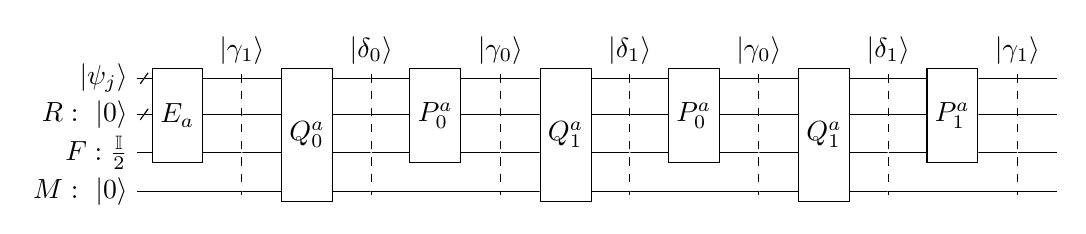
\begin{tikzpicture}
\begin{yquant*}
qubit {$\ket{\psi_j}$}  s;
qubit {$R:\ \ket{0}$} anc;
qubit {$F: \frac{\mathbb{I}}{2}$} f;
qubit {$M:\ \ket{0}$} m;
slash s;
slash anc;
hspace {0.1cm} -;
box {$E_a$} (s,anc,f);
["$\ket{\gamma_1}$"]
barrier (-);
box {$Q^a_0$} (s,anc,f, m);
["$\ket{\delta_0}$"]
barrier (-);
box {$P^a_0$} (s,anc,f);
["$\ket{\gamma_0}$"]
barrier (-);
box {$Q^a_1$} (s,anc,f, m);
["$\ket{\delta_1}$"]
barrier (-);
box {$P^a_0$} (s,anc,f);
["$\ket{\gamma_0}$"]
barrier (-);
box {$Q^a_1$} (s,anc,f, m);
["$\ket{\delta_1}$"]
barrier (-);
box {$P^a_1$} (s,anc,f);
["$\ket{\gamma_1}$"]
barrier (-);
\end{yquant*}
\end{tikzpicture}
\caption{A successfully completed rejection procedure. The same BSI-QPE registers $R, F$ is reused by $E_{ae}$ and every $P_s^{ae}$ and $Q_s^{ae}$; the qubit $M$ is reused by every $Q_s^{ae}$. This circuit corresponds to a term in $\mathcal{B}(2)[\rho]$ for $\{s_n\}=\{1,1\}$ and, within a single invariant subspace $\lambda$ (see Section~\ref{section:rejection}), occurs with probability $(1-p^{aej}_{\lambda})^4(p^{aej}_{\lambda})^2$. The state labels at the barriers denote the corresponding states of each invariant subspace.}
\label{fig:fullcircuit}
\end{figure*}

The iterative process proceeds as follows after measuring $s=0$ (reject) from the initial $Q_s^{ae}$ measurement: 
\begin{enumerate}
    \item Measure $P_s^{ae}$
        \begin{enumerate}
            \item If $s=1$ \textbf{terminate} as the state has returned to the approximate energy of the initial state.
            \item If $s=0$ continue.
        \end{enumerate}
    \item Measure $Q_s^{ae}$
    \item Repeat up to a maximum of $n^*$ iterations
\end{enumerate}


Let us consider the action of the rejection process on each eigenvector $\ket{\psi_j}$ of $H$. To handle the mixed initial state of $F$, purify $\frac{\mathbb{I}}{2}$ as $\ket{\Phi}_{FF'}=\frac{1}{\sqrt{2}}\sum_f\ket{f}_F\ket{f}_{F'}$, where the reference $F'$ is never acted upon. Conditioned on the outcome $(a,e)$, the corresponding pure post-measurement state is
\begin{equation}
    \frac{(E_{ae}\otimes\mathbb I_{F'})\ket{\psi_j}\ket{0}_R\ket{\Phi}_{FF'}\ket{0}_M}
    {\|(E_{ae}\otimes\mathbb I_{F'})\ket{\psi_j}\ket{0}_R\ket{\Phi}_{FF'}\ket{0}_M\|}
    = \sum_{\lambda} c_{\lambda}^{aej}\ket{\gamma_1^{ae \lambda}}.
\end{equation}
Tracing out $F'$ recovers the physical evolution from $\frac{\mathbb{I}}{2}$. Because $P_1^{ae}E_{ae}=E_{ae}$, this state is a $+1$ eigenstate of $P_1^{ae}$ (with all projectors implicitly extended by $\mathbb I_{F'}$). Furthermore, $P_1^{ae}$ commutes with $P^{ae}_1Q^{ae}_0P^{ae}_1$, so the two operators are jointly diagonalizable and the expansion above may be taken in their joint eigenstates. The untouched reference is absorbed into the degeneracy label $\lambda$.
Writing the eigenvalue of $\ket{\gamma^{ae\lambda}_1}$ as $1-p^{ae\lambda}$, we have: \begin{align}1-p^{ae\lambda}&=\bra{\gamma^{ae\lambda}_1}P^{ae}_1Q^{ae}_0P^{ae}_1\ket{\gamma^{ae\lambda}_1} \\&=\|Q^{ae}_0P^{ae}_1\ket{\gamma^{ae\lambda}_1}\|^2\\ &= 1-\|Q^{ae}_1\ket{\gamma^{ae\lambda}_1}\|^2
\end{align}
so $p^{ae\lambda} = \|Q^{ae}_1\ket{\gamma^{ae\lambda}_1}\|^2$, and the probability of accepting the update is given by the mixture $p_{aej} = \sum_{\lambda}|c^{aej}_{\lambda}|^2p^{ae\lambda}$. Therefore, for each $\lambda$ with $p^{ae\lambda} \in (0,1)$ we can define the following 2D invariant subspace (we have suppressed the $ae\lambda$ labels for the remainder of this section for clarity, writing $\ket{\gamma_1} = \ket{\gamma^{ae\lambda}_1}$ and $p = p^{ae\lambda}$):
\begin{align}
    \ket{\delta_0} &= \frac{Q^{ae}_0P^{ae}_1\ket{\gamma_1}}{\sqrt{1-p}} &\ket{\delta_1} &= \frac{Q^{ae}_1P^{ae}_1\ket{\gamma_1}}{\sqrt{p}} \\
    \ket{\gamma_0} &= \frac{P^{ae}_0Q^{ae}_0\ket{\delta_0}}{\sqrt{p}} &\ket{\gamma_1} &= \frac{P^{ae}_1Q^{ae}_0\ket{\delta_0}}{\sqrt{1-p}}
\end{align}
From these definitions the following relations can be deduced:
\begin{align}
\begin{split}
\label{eq:deltagamma0}
    P^{ae}_1 \ket{\gamma_1} &= (Q^{ae}_0+Q^{ae}_1)P^{ae}_1 \ket{\gamma_1}\\
    &= Q^{ae}_0P^{ae}_1 \ket{\gamma_1}+Q^{ae}_1P^{ae}_1 \ket{\gamma_1}\\
    &= \sqrt{1-p} \ket{\delta_0} + \sqrt{p}\ket{\delta_1}\\
    Q^{ae}_0\ket{\delta_0} &= \sqrt{p} \ket{\gamma_0} + \sqrt{1-p} \ket{\gamma_1}
\end{split}
\end{align}
As $P^{ae}_1 \ket{\gamma_1} = \ket{\gamma_1}$ and $Q^{ae}_0\ket{\delta_0} = \ket{\delta_0}$ we can simplify the above and then through substitution deduce the remaining relations:
\begin{align}
\begin{split}
\label{eq:deltagamma1}
        \ket{\delta_1} &= -\sqrt{1-p} \ket{\gamma_0} + \sqrt{p} \ket{\gamma_1}\\
    \ket{\gamma_0} &= \sqrt{p} \ket{\delta_0} - \sqrt{1-p}\ket{\delta_1}
\end{split}
\end{align}
Therefore it is clear that each measurement transitions the state from one of $\ket{\delta_i}$ to one of $\ket{\gamma_i}$ or vice versa, whilst remaining within the same 2D invariant subspace. As the subspaces corresponding to different $\lambda$ are mutually orthogonal (which follows from the orthogonality of the $\ket{\gamma^{ae\lambda}_1}$ together with the relations above) and each is preserved by both measurements, the subspaces do not mix at any point during the rejection process. The probability of these transitions are trivially deduced from \eqref{eq:deltagamma0} and \eqref{eq:deltagamma1}, and can be seen in Fig.~\ref{fig:transitions}.
\begin{figure}
    \centering
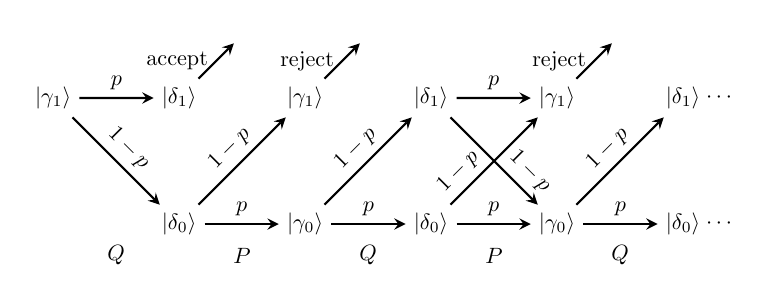
\begin{tikzpicture}[node distance=2cm, >=stealth, thick, scale=0.8, transform shape]
    \node (g-1t) at (0,2) {$|\gamma_1\rangle$};
    \node (s0t)  at (2,2) {$|\delta_1\rangle$};
    \node (s0)  at (2,0) {$|\delta_0\rangle$};
    \node (g0)  at (4,0) {$|\gamma_0\rangle$};
    \node (s1)  at (6,0) {$|\delta_0\rangle$};
    \node (g1)  at (8,0) {$|\gamma_0\rangle$};
    \node (s2)  at (10,0) {$|\delta_0\rangle$};
    \node (...1) at (10.6,0) {$\cdots$};
    \node (...2) at (10.6,2) {$\cdots$};
    
    \node (a) at (3,3) {};
    \node (r1) at (5,3) {};
    \node (r2) at (9,3) {};
    
    \node (g1t) at (4,2) {$|\gamma_1\rangle$};
    \node (s1t) at (6,2) {$|\delta_1\rangle$};
    \node (g2t) at (8,2) {$|\gamma_1\rangle$};
    \node (s2t) at (10,2) {$|\delta_1\rangle$};
    
    % Transitions
    \draw[->] (s0) -- node[above] {$p$} (g0);
    \draw[->] (g0) -- node[above] {$p$} (s1);
    \draw[->] (s1) -- node[above] {$p$} (g1);
    \draw[->] (g1) -- node[above] {$p$} (s2);
    
    \draw[->] (s0) -- node[above,sloped] {$1-p$} (g1t);
    \draw[->] (g0) -- node[above ,sloped] {$1-p$} (s1t);
    \draw[->] (s1) -- node[above left,sloped] {$1-p$} (g2t);
    \draw[->] (s1t) -- node[above] {$p$} (g2t);
    \draw[->] (g-1t) -- node[above] {$p$} (s0t);
    
    \draw[->] (s1t) -- node[above right,sloped] {$1-p$} (g1);
    \draw[->] (g1) -- node[above ,sloped] {$1-p$} (s2t);
    \draw[->] (g-1t) -- node[above ,sloped] {$1-p$} (s0);

    \draw[->] (s0t) -- node[left] {accept} (a);
    \draw[->] (g1t) -- node[left] {reject} (r1);
    \draw[->] (g2t) -- node[left] {reject} (r2);

    % Labels
    \node at (1,-0.5) {$Q$};
    \node at (3,-0.5) {$P$};
    \node at (5,-0.5) {$Q$};
    \node at (7,-0.5) {$P$};
    \node at (9,-0.5) {$Q$};
\end{tikzpicture}
    \caption{Markov chain showing the transition probability between the 4 states of a single invariant subspace $\lambda$ (with $p = p^{ae\lambda}$) upon each projective measurement. The full rejection process is a mixture of such chains weighted by $|c^{aej}_{\lambda}|^2$.}
    \label{fig:transitions}
\end{figure}

From this we can calculate the probability of attempting to reject and then failing the rejection process within a single invariant subspace to be $p(1-p)(p^2 +(1-p)^2)^{n^*}$. As the subspaces do not mix, the overall failure probability $p_a^{fail}$ is the corresponding mixture over subspaces (reinstating the suppressed labels):
\begin{equation}
   p_{aej}^{fail} =  \sum_{\lambda}|c^{aej}_{\lambda}|^2p^{ae\lambda}(1-p^{ae\lambda})((p^{ae\lambda})^2 +(1-p^{ae\lambda})^2)^{n^*}
\end{equation}
For all $p \in [0,1]$ we have: 
\begin{equation}
    p(1-p)(p^2 +(1-p)^2)^{n^*} \leq \frac{1}{2(n^*+1)} \left(\frac{n^*}{n^*+1}\right)^{n^*}
\end{equation}
Therefore, as $\sum_{\lambda}|c^{aej}_{\lambda}|^2=1$ we have:
\begin{equation}
    \label{eq:probabilty_of_rejection}
   p_{aej}^{fail} \leq \frac{1}{2(n^*+1)} \left(\frac{n^*}{n^*+1}\right)^{n^*} \leq \frac{1}{2n^*}
\end{equation}
If the rejection process fails then the whole algorithm fails irrecoverably and must be restarted from the original initial state.

\label{section:rejection}
\begin{table*}
\caption{Notation used throughout the analysis.}
\label{tab:notation}
\begin{ruledtabular}
\begin{tabular}{llp{0.62\textwidth}}
Symbol & Introduced & Meaning \\
\colrule
$R,F,M$ & Sec.~\ref{section:algorithm} & persistent $\eta$-qubit energy-index register, window qubit, acceptance-rotation qubit \\
$F'$ & Sec.~\ref{section:rejection} & purifying reference for $F$ (never acted upon) \\
$\omega_j$ & Eq.~\eqref{eq:omegadef} & eigenenergy in phase-estimation bins, $\omega_j = \frac{2^{\eta}t}{2\pi}E_j$ \\
$(a,e)$ / $(b,d)$ & Figs.~\ref{fig:Ecircuit},\,\ref{fig:LQ_circuit} & initial / proposed energy record measured from $(R,F)$ \\
$s$, $s_i$ & Fig.~\ref{fig:Qcircuit} & accept/reject outcome of $Q^{ae}_s$; outcomes during the rewind loop \\
$p_i, q_i$; $z$ & Eq.~\eqref{eq:Arho} ff. & ket/bra paths of the $R$ register; final traced $R$ index \\
$j,k,l,m$ & Lemma~\ref{lemma:1} & Hamiltonian eigenindices of matrix elements $\bra{\psi_m}\cdot[\ket{\psi_j}\bra{\psi_k}]\ket{\psi_l}$ \\
$G^{pq}_j$, $\tilde G^{pq}_j$ & Eqs.~\eqref{eq:G},\,(\ref{eq:decomposealpha}--\ref{eq:decomposealpha3}) & BSI-QPE block; band-limited (truncated) version, bandwidth $\mu$ \\
$\eta, t, \mu, \nu, r, b, n^*$ & Secs.~\ref{section:boostedphaseestimation},\,\ref{section:algorithm} & ancilla count; evolution time $t=\frac{1}{16\|H\|}$; truncation bandwidth; tail decay rate; window parameters; rewinding cap \\
$\epsilon_{\Delta}$ & Eq.~\eqref{eq:decomposealpha3} & total truncated tail weight, $O(\sqrt{2^{\eta}}e^{-\nu\mu})$ \\
$\mathcal{A}, \mathcal{B}(n), \mathcal{C}$ & Sec.~\ref{subsec:cptp} & accept / successful-rejection / failed-rejection channels \\
$\mathfrak{E}, \mathcal{P}_S, \mathcal{Q}_S, \mathcal{L}$ & Sec.~\ref{subsec:transfer} & CP maps of the constituent measurements \\
$\mathcal{M}_{\sigma}, \mathcal{M}^{\dagger}, \mathcal{M}^*_{\sigma}$ & Sec.~\ref{subsec:aqdb} & $\sigma^{1/2}$-weighted map, adjoint map, $\sigma$-weighted adjoint \\
$\tilde{\ }$ (on maps) & Sec.~\ref{subsec:cptp} & the same map built from the truncated $\tilde G^{pq}_j$ \\
$f_{abde}$, $\kappa_{abde}$ & Eqs.~\eqref{eq:kappadef},\,\eqref{eq:fdef} & acceptance probability and its record-difference argument \\
$\bar g^{ae}$ & Eq.~\eqref{eq:gbar-definition} & summed-history amplitude of the rewind loop \\
\end{tabular}
\end{ruledtabular}
\end{table*}
\section{Why it works}
\label{section:why}
The classical Metropolis-Hastings algorithm works by constructing a Markov Chain through proposing and accepting/rejecting moves with probabilities determined by the energy difference between the initial and modified states. The transition matrix of this Markov chain is in detailed balance with respect to the Gibbs state, implying that the Gibbs state is a fixed point of the Markov chain. As Markov chain is also ergodic, it is known that it must have a single unique fixed point and converge towards it. Therefore, the Markov chain converges to the Gibbs state.

In the quantum Metropolis algorithm we similarly construct a quantum Markov chain by proposing and accepting or rejecting moves based on energy differences. Because the energy differences cannot be resolved exactly, we cannot prove exact detailed balance and instead use a notion of approximate quantum detailed balance that incorporates additive errors from the nonzero, exponentially suppressed tails of BSI-QPE. This establishes that the Gibbs state is approximately invariant. Closeness of the actual fixed point additionally depends on the mixing properties of the channel, as made explicit below. Choosing the update set $\{C\}$ to be universal ensures ergodicity \cite{Temme_2011}.

\subsection{Main result and proof strategy}
\label{subsec:main}
The destination of this section is the following statement; every quantity appearing in it has already been introduced ($\nu$ in Eq.~\eqref{eq:scaling}, $\mu$ in Eqs.~(\ref{eq:decomposealpha}--\ref{eq:decomposealpha3}), $n^*$ in Section~\ref{section:rejection}), and Table~\ref{tab:notation} collects the notation.
\begin{theorem}[Main result]
\label{theorem:main}
Let $\mathcal{E}$ be one update round of the quantum Metropolis algorithm of Section~\ref{section:algorithm}, implemented with $\eta$ ancillas, evolution time $t = \frac{1}{16\|H\|}$, rewinding cap $n^*$, an update measure satisfying $d\mu(C)=d\mu(C^{\dagger})$, and window functions satisfying the conditions of Appendix~\ref{section:appendix} with truncation bandwidth $\mu = O(\frac{1}{\nu}\log n^*)$, $\mu < \frac{2^{\eta}}{96\pi}$. Then
\begin{equation}
   \|\mathcal{E}[\sigma_G] - \sigma_G\|_* = O\left(\max\left( n^{*\frac{7}{2}}\sqrt{\frac{\beta\|H\| }{2^{\eta}}}\mu^{\frac{3}{2}},\frac{1}{n^*}\right)\right).
\end{equation}
If, in addition, $\mathcal{E}$ is strictly trace-norm contracting with factor $k<1$, then $\mathcal{E}$ has a unique fixed point $\sigma^*$, is approached exponentially fast, and $\|\sigma^*-\sigma_G\|_* \leq \frac{1}{1-k}\|\mathcal{E}[\sigma_G] - \sigma_G\|_*$ (Theorem~\ref{theorem:error_bound}).
\end{theorem}

The proof occupies the remainder of this section, with the heavier verifications deferred to Appendices~\ref{app:perturbation}--\ref{app:rejectproof}. It consists of four moves, applied first to the acceptance channel $\mathcal{A}$ and then, with measurement \emph{histories} in place of single outcomes, to each rejection channel $\mathcal{B}(n)$:
\begin{enumerate}
    \item \textbf{Truncate.} Replace $\hat\alpha, \hat\beta$ by their band-limited versions $\tilde\alpha, \tilde\beta$ (Lemma~\ref{lemma:0}). Lemma~\ref{lemma:3} converts this operator-norm replacement into a diamond-norm error $O(\epsilon_{\Delta}/\sqrt{2^{\eta}})$ per measurement, so the detailed-balance computation may be carried out with strictly band-limited $\tilde G^{pq}_j$, whose support ties every measurement record to the energies involved (Lemma~\ref{lemma:support}).
    \item \textbf{Reverse paths.} Each measurement branch $c$ of the truncated map has a reversal partner $c'$ (an involution: $a \leftrightarrow b$, $e \leftrightarrow d$, register paths reversed, $z \mapsto 2^{\eta}-z$) such that the branch of the $\sigma_G$-adjoint at $c'$ has exactly the same amplitude structure as the branch of the map at $c$. This is where $d\mu(C) = d\mu(C^{\dagger})$ and, for $\mathcal{B}(n)$, the summed-history reversal (Lemma~\ref{lemma:summed-history-reversal}) enter.
    \item \textbf{Reweight.} The reversed branch carries $f_{c'}$ and Boltzmann factors $e^{-\frac{\beta}{2}(E_l+E_m)}$ where the original carried $f_c$ and $e^{-\frac{\beta}{2}(E_j+E_k)}$; because the records pin the energies to within $O(\mu)$ bins, the two agree up to $(1+u)^2$ with $|u| = O(\frac{\beta\mu}{2^{\eta}t})$ (Lemma~\ref{lemma:reweight}). This is an approximate, branchwise $\sigma_G$-detailed-balance condition, formalised by Lemma~\ref{lemma:1}.
    \item \textbf{Assemble.} Theorem~\ref{theorem:quantumapproximatedeatildedbalance} sums the branch errors; the failure channel $\mathcal{C}$ is not balanced but merely small, $O(\frac{1}{n^*})$ by Eq.~\eqref{eq:probabilty_of_rejection}; and Theorem~\ref{theorem:error_bound} converts approximate stationarity into closeness of the fixed point under the contraction assumption.
\end{enumerate}
\subsection{Warm-up: exact detailed balance for ideal phase estimation}
\label{subsec:warmup}
Before the full analysis it is instructive to run the argument in an idealised limit in which every step is exact. Suppose (i) every eigenenergy falls exactly on the phase-estimation grid, $\omega_j \in \mathbb{Z}$ for all $j$, and (ii) the windows are taken constant, $\alpha(x) = \cos\theta$, $\beta(x) = \sin\theta$, so that $\hat\alpha(x)$ and $\hat\beta(x)$ are supported entirely at $x = 0$; equivalently, $\mu = 0$ with $\epsilon_{\Delta} = 0$. (By the Remark at the end of Section~\ref{section:boostedphaseestimation}, this is exactly the regime in which unboosted QPE would already suffice; the point of this subsection is that everything the full proof must control is a controlled deviation from this limit.)

In this limit the support constraints of Lemma~\ref{lemma:support} hold with $\mu = 0$ and therefore become exact equalities: a nonzero acceptance branch forces $p_1 = q_1 = p_2 = 0$, an initial record $a = (-1)^e\omega_j = (-1)^e\omega_k$, and a proposed record $b = (-1)^d\omega_m = (-1)^d\omega_l$. Consequently $\kappa_{abde} = (-1)^db - (-1)^ea = \omega_m - \omega_j$ exactly, and the acceptance probability of Eq.~\eqref{eq:fdef} is exactly the classical Metropolis rule, $f_{abde} = \min(1, e^{-\beta(E_m-E_j)})$. The reweighting identity of Lemma~\ref{lemma:reweight} then holds with $u \equiv 0$: it reduces to the elementary detailed-balance identity
\begin{equation}
\begin{split}
    e^{-\beta E_j}\min(1, e^{-\beta(E_m - E_j)}) &= \min(e^{-\beta E_j}, e^{-\beta E_m}) \\
    &= e^{-\beta E_m}\min(1, e^{-\beta(E_j - E_m)}),
\end{split}
\end{equation}
while the path reversal $(a,b,d,e) \mapsto (b,a,e,d)$ maps admissible records to admissible records and $d\mu(C) = d\mu(C^{\dagger})$ supplies the proposal symmetry. Lemma~\ref{lemma:1} therefore applies with $\epsilon_m = 0$ and yields \emph{exact} stationarity of the acceptance channel: $\mathcal{A}^*_{\sigma_G}[\mathbb{I}] = \mathcal{A}[\sigma_G]$.

The rejection channels are handled the same way. The Marriott--Watrous analysis of Section~\ref{section:rejection} is exact in all cases and needs no idealisation. In the ideal limit the final traced register index is forced to $z = 0$ (its support bound $|z|_{2^{\eta}} \leq (4n+6)\mu$ collapses), so the acceptance rotations are not dragged by the reversal at all and the history-reversal symmetry of the rewind loop (Lemma~\ref{lemma:summed-history-reversal}) gives, again with $u \equiv 0$, exact stationarity $\mathcal{B}^*_{\sigma_G}(n)[\mathbb{I}] = \mathcal{B}(n)[\sigma_G]$ for every $n$. The only unbalanced piece is the failure channel, so Theorem~\ref{theorem:quantumapproximatedeatildedbalance} gives, in the ideal limit,
\begin{equation}
    \|\mathcal{E}[\sigma_G] - \sigma_G\|_* \leq 2\|\mathcal{C}[\sigma_G]\|_* \leq \frac{1}{n^*}.
\end{equation}

The remainder of this section controls the three deviations of the real algorithm from this ideal, summarised in Table~\ref{tab:whatbreaks}: the exponentially suppressed but nonzero window tails ($\epsilon_{\Delta}$), the nonzero bin width ($\mu > 0$, producing the multiplicative $(1+u)$ factors), and the $z$-drift of the acceptance rotations under path reversal (producing the $\mu^{3/2}$ term).
\begin{table*}
\caption{The ideal-QPE limit versus the real algorithm.}
\label{tab:whatbreaks}
\begin{ruledtabular}
\begin{tabular}{lll}
Idealisation & Real deviation & Controlled by \\
\colrule
$\hat\alpha, \hat\beta$ supported at a point & tails of total weight $\epsilon_{\Delta}$ & Lemma~\ref{lemma:0} $+$ Lemma~\ref{lemma:3} $+$ Lemma~\ref{lemma:composition} \\
records determine energies exactly & only to within $O(\mu)$ bins & Lemma~\ref{lemma:support} $+$ Lemma~\ref{lemma:reweight} ($(1+u)$ factors) \\
reversal leaves $W_{abde}$ untouched ($z=0$) & controls dragged by $|z| \leq (4n+6)\mu$ & Lemma~\ref{lemma:wdrift} ($W$-drift) \\
\end{tabular}
\end{ruledtabular}
\end{table*}
\subsection{Approximate quantum detailed balance}
\label{subsec:aqdb}
Below we present our modified formulation of approximate quantum detailed balance:

For any completely positive map $\mathcal{M}$ ($\mathcal{M}[\rho] =\sum_{j}  A_{j}\rho  A^{\dagger}_{j}$) and density matrix $\sigma$, we define $\mathcal{M}_{\sigma}[\rho] =\sum_{j}  A_{j}\sigma^{\frac{1}{2}}\rho\sigma^{\frac{1}{2}}  A^{\dagger}_{j}$, $\mathcal{M}^{\dagger}[\rho] = \sum_j A^{\dagger}_j \rho A_j$ and $ \mathcal{M}^*_{\sigma}[\rho] = \sum_{j} \sigma^{\frac{1}{2}}A^{\dagger}_{j}\rho A_{j}\sigma^{\frac{1}{2}} = \sigma^{\frac{1}{2}}\mathcal{M}^{\dagger}[\rho]\sigma^{\frac{1}{2}}$.
\begin{lemma}[Branchwise approximate $\sigma$-detailed balance]
\label{lemma:1}
Let $\mathcal{M}$ and $\mathcal{M'}$ be a completely positive maps on $d$-dimensional density matrices admitting the same decomposition $\mathcal{M} = \sum_{c\in\mathcal{X}} \mathcal{M}_c$, $\mathcal{M'} = \sum_{c\in\mathcal{X}} \mathcal{M'}_c$ into completely positive maps $\mathcal{M}_c$ and $\mathcal{M}'_c$, and let $\sigma = \sum_j \sigma_j \ket{\psi_j}\bra{\psi_j}$ be a density matrix diagonal in the orthonormal basis $\{\ket{\psi_j}\}$. Suppose there exists a bijection $c \mapsto c'$ of $\mathcal{X}$ such that, for every $j,c,l,m$,
\begin{multline}
    \bra{\psi_m}\mathcal{M}'^*_{c'\sigma}[\ket{\psi_j}\bra{\psi_j}]\ket{\psi_l}
    =\\(1+u^{jc}_m)(1+ u^{jc}_l)
    \bra{\psi_m}\mathcal{M}_{c\sigma}[\ket{\psi_j}\bra{\psi_j}]\ket{\psi_l}
    \label{eq:approximate_quantum_detailed_balance_condition}
\end{multline}
where the $u^{jc}_l$ are real and satisfy $|u^{jc}_l| \leq \epsilon_m$. Then:
 \begin{equation}
    \|\mathcal{M}'^*_{\sigma}[\mathbb{I}]-\mathcal{M}[\sigma] \|_* \leq (2\epsilon_m+\epsilon_m^2)\|\mathcal{M}[\sigma]\|_* 
\end{equation}
where $\|\cdot\|_*$ is trace-norm.
\end{lemma}

\begin{proof}
    By definition $\mathcal{M}[\sigma]=\mathcal{M}_{\sigma}[\mathbb{I}]$. By linearity and the bijectivity of $c \mapsto c'$:
    \begin{equation}
        \mathcal{M}'^*_{\sigma}[\mathbb{I}] = \sum_{j,c}\mathcal{M}'^*_{c\sigma}[\ket{\psi_j}\bra{\psi_j}] = \sum_{j,c}\mathcal{M}'^*_{c'\sigma}[\ket{\psi_j}\bra{\psi_j}]
    \end{equation}
    Define $N^{jc} = \mathcal{M}_{c\sigma}[\ket{\psi_j}\bra{\psi_j}]$ and $D^{jc}=\sum_l(1+u_l^{jc})\ket{\psi_l}\bra{\psi_l}$. Equation~\eqref{eq:approximate_quantum_detailed_balance_condition} is then the operator identity $\mathcal{M}'^*_{c'\sigma}[\ket{\psi_j}\bra{\psi_j}]=D^{jc}N^{jc}D^{jc}$. Moreover, $N^{jc}$ is positive semidefinite as $\mathcal{M}_c$ is completely positive, so that $\mathcal{M}_{\sigma}[\mathbb{I}] = \sum_{j,c}N^{jc}$. Writing $V^{jc} = D^{jc}-\mathbb{I}$, which satisfies $\|V^{jc}\|\leq\epsilon_m$, we have:
    \begin{equation}
        D^{jc}N^{jc}D^{jc} - N^{jc} = V^{jc}N^{jc} + N^{jc}V^{jc} + V^{jc}N^{jc}V^{jc}
    \end{equation}
    By H\"older's inequality each term is bounded in trace-norm as:
    \begin{equation}
        \|V^{jc}N^{jc}\|_* \leq \|V^{jc}\|\|N^{jc}\|_* \leq \epsilon_m Tr[N^{jc}]
    \end{equation}
    and similarly for the remaining terms. Therefore, by the triangle inequality:
    \begin{align}
        \|\mathcal{M}'^*_{\sigma}[\mathbb{I}]-\mathcal{M}_\sigma[\mathbb{I}]\|_* &\leq \sum_{j,c}\left(\|D^{jc}N^{jc}D^{jc}-N^{jc}\|_*\right)\\
        &\leq (2\epsilon_m+\epsilon_m^2)\sum_{j,c}Tr[N^{jc}] 
    \end{align}
    Finally, as each $N^{jc}$ is positive semidefinite:
    \begin{equation}
        \sum_{j,c}Tr[N^{jc}] = Tr[\mathcal{M}_{\sigma}[\mathbb{I}]] = Tr[\mathcal{M}[\sigma]] = \|\mathcal{M}[\sigma]\|_*
    \end{equation}
\end{proof}
\begin{remark}[Relation to $\sigma$-detailed balance]
Lemma~\ref{lemma:1} is an approximate, branch-resolved form of the quantum detailed balance conditions used in the Gibbs-sampler literature. The map $\mathcal{M}^*_{\sigma}$ is the adjoint of $\mathcal{M}$ with respect to the $\sigma^{1/2}$-weighted (KMS-type) inner product $\braket{X,Y}_{\sigma} = Tr[X^{\dagger}\sigma^{\frac{1}{2}}Y\sigma^{\frac{1}{2}}]$, and exact quantum detailed balance of a channel is self-adjointness in this inner product \cite{temme2010chi,chen2023quantumthermalstatepreparation}. Setting $u^{jc}_l \equiv 0$ and $\mathcal{M}' = \mathcal{M}$ in Eq.~\eqref{eq:approximate_quantum_detailed_balance_condition} recovers exactly that notion, branch-paired by $c \mapsto c'$; the lemma weakens it multiplicatively, per branch, which is what an imperfect energy estimate can actually deliver.
\end{remark}
\begin{theorem}[Approximate Quantum Detailed Balance]
\label{theorem:quantumapproximatedeatildedbalance}
Given a completely positive trace preserving map $\mathcal{E}$ on $d$-dimensional density matrices constructed from a sum of completely positive maps $\mathcal{M}_j$:
\begin{equation}
    \mathcal{E}[\rho] = \sum_j \mathcal{M}_j[\rho]
\end{equation}
If for every $\mathcal{M}_j$ and the same given density matrix $\sigma$ we have:
\begin{equation}
    \|\mathcal{M}^*_{j\sigma}[\mathbb{I}]-\mathcal{M}_{j}[\sigma]\|_* \leq \epsilon^j
\end{equation}
(as is provided by Lemma~\ref{lemma:1} with $\epsilon^j = (2\epsilon^j_m+(\epsilon^j_m)^2)\|\mathcal{M}_j[\sigma]\|_*$), then we have:
\begin{equation}
     \|\mathcal{E}[\sigma]-\sigma\|_* \leq \sum_j\min\left(\epsilon^j, 2\|\mathcal{M}_j[\sigma]\|_*\right)
\end{equation}
\end{theorem}
\begin{proof}
    By the triangle inequality we have:
    \begin{equation}
        \|\mathcal{E}^*_{\sigma}[\mathbb{I}]-\mathcal{E}[\sigma]\|_* \leq \sum_j \|\mathcal{M}^*_{j\sigma}[\mathbb{I}]-\mathcal{M}_{j}[\sigma]\|_*
    \end{equation}
    As $\mathcal{E}$ is trace-preserving, we know that:
    \begin{equation}
        \mathcal{E}^*_{\sigma}[\mathbb{I}] = \sum_{j} \sigma^{\frac{1}{2}}A^{\dagger}_{j} A_{j}\sigma^{\frac{1}{2}} = \sigma
    \end{equation}
    Therefore,
    \begin{equation}
        \|\sigma - \mathcal{E}[\sigma]\|_* \leq \sum_j \|\mathcal{M}^*_{j\sigma}[\mathbb{I}]-\mathcal{M}_{j}[\sigma]\|_*
    \end{equation}
    By assumption we have that for all $j$:
    \begin{equation}
        \|\mathcal{M}^*_{j\sigma}[\mathbb{I}]-\mathcal{M}_{j}[\sigma]\|_* \leq \epsilon^j
    \end{equation}
    Further, as both
$\mathcal{M}_{j,\sigma}^{*}[\mathbb{I}]$ and
$\mathcal{M}_j[\sigma]$ are positive semidefinite:
    \begin{align}
        \|\mathcal{M}^*_{j\sigma}[\mathbb{I}]\|_* &= Tr\left[\sum_l \sigma^{\frac{1}{2}} K_{jl}^{\dagger} \mathbb{I} K_{jl} \sigma^{\frac{1}{2}}\right]\\
        &= Tr\left[\sum_l K_{jl}\sigma K_{jl}^{\dagger}\right]\\
        &= \|\mathcal{M}_{j}[\sigma]\|_*
    \end{align}
    Therefore,
    \begin{equation}
         \|\mathcal{M}^*_{j\sigma}[\mathbb{I}]-\mathcal{M}_{j}[\sigma]\|_* \leq 2\|\mathcal{M}_{j}[\sigma]\|_*
    \end{equation}
    Hence,
    \begin{equation}
        \|\sigma-\mathcal{E}[\sigma]\|_* \leq \sum_j \min \left(\epsilon^j, 2\|\mathcal{M}_{j}[\sigma]\|_*\right)
    \end{equation}
\end{proof}
\subsection{The update round as a completely positive map}
\label{subsec:cptp}
\begin{widetext}
To demonstrate an update round $\mathcal{E}$ of the Quantum Metropolis algorithm is in approximate quantum detailed balance with respect to the Gibbs state $\sigma_G$, we must express it as a completely positive trace preserving map:
\begin{equation}
    \mathcal{E}[\rho] = \mathcal{A}[\rho] + \sum_{n=0}^{n^*} \mathcal{B}(n)[\rho] + \mathcal{C}[\rho]
\end{equation}
where $\mathcal{A}$ corresponds to acceptance, $\mathcal{B}(n)$ to successful rejection after $n$ iterations and $\mathcal{C}$ to failing to reject after $n^*$ iterations. Let $\Omega_{RFM} =\ket{0}\bra{0}_R\otimes \frac{\mathbb{I}_F}{2}\otimes\ket{0}\bra{0}_M$ denote the initial state of the persistent ancillas. All occurrences of $E_{ae}$, $P_s^{ae}$, $Q_s^{ae}$ and $L_b^{ade}$ below act on this common ancillary space, with identities on any register on which a given operator acts trivially. Then
\begin{equation}
    \mathcal{A}[\rho] = \int  Tr_{RFM}\bigg[\sum_{a,b,d,e}L_b^{ade} E_{ae} ( \rho\otimes \Omega_{RFM}) 
     E_{ae}L^{ade\dagger}_b\bigg]d\mu(C)
\end{equation}
\begin{equation}
    \mathcal{B}(n)[\rho] = \int Tr_{RFM}\bigg[\sum_{a,e,\{s\}}P^{ae}_1Q^{ae}_{s_n}\ldots P^{ae}_0Q^{ae}_{s_1}P^{ae}_0Q^{ae}_0E_{ae} ( \rho\otimes \Omega_{RFM})E_{ae}Q^{ae}_0P^{ae}_0Q^{ae}_{s_1}P^{ae}_0\ldots Q^{ae}_{s_n}P^{ae}_1\bigg]d\mu(C)
\end{equation}
\begin{equation}
    \mathcal{C}[\rho] = \rho_0 \int Tr\bigg[\sum_{a,e,\{s\}}P^{ae}_0Q^{ae}_{s_{n^*}}\ldots P^{ae}_0Q^{ae}_{s_1}P^{ae}_0Q^{ae}_0E_{ae} ( \rho\otimes \Omega_{RFM})E_{ae}Q^{ae}_0P^{ae}_0Q^{ae}_{s_1}P^{ae}_0\ldots Q^{ae}_{s_{n^*}}P^{ae}_0\bigg]d\mu(C) 
\end{equation}
where $\rho_0$ is the initial state the overall Metropolis algorithm was started from. 
To use Theorem~\ref{theorem:quantumapproximatedeatildedbalance}, we must bound $\|\mathcal{A}^*_{\sigma_G}[\mathbb{I}]-\mathcal{A}[\sigma_G]\|_*$ and $\|\mathcal{B}^*_{\sigma_G}(n)[\mathbb{I}]-\mathcal{B}(n)[\sigma_G]\|_*$, which we do by verifying the branch-wise condition \eqref{eq:approximate_quantum_detailed_balance_condition} of Lemma~\ref{lemma:1}. To do so we will consider approximations to $\mathcal{A}$ and $\mathcal{B}(n)$ in which we have substituted $\tilde \alpha, \tilde \beta$ for $\hat \alpha, \hat \beta$. Under this substitution $G^{pq}_j$ becomes $\tilde G^{pq}_j$ such that $\|\tilde G^{pq}_j\| =0$ for all $|p-q\pm\omega_{j}|_{2^{\eta}} > \mu$. Then using Lemma~\ref{lemma:3} we will show that $\|\tilde{\mathcal{A}}-\mathcal{A}\|_{\diamond} \leq \epsilon$ and $\|\tilde{\mathcal{B}}(n)-\mathcal{B}(n)\|_{\diamond} \leq \epsilon$, and hence transfer the bounds from the approximated maps to the true maps. We will not evaluate Lemma~\ref{lemma:1} for $\mathcal{C}$, but rather bound its contribution in Theorem~\ref{theorem:quantumapproximatedeatildedbalance} by its trace-norm.
\end{widetext}
\subsection{Truncation transfer}
\label{subsec:transfer}
\begin{lemma}[Measurement perturbation in diamond norm]
\label{lemma:3}
Let $\{D_s\}_{s\in S}$ be mutually orthogonal projectors satisfying $\sum_{s\in S} D_s \leq \mathbb{I}$. Given a unitary $U$, define the projective measurement $K_s = U^{\dagger}D_s U$ and CP map $\mathcal{K}[\rho] = \sum_{s \in S} K_s\rho K_s^{\dagger}$. Further, given an operator $\tilde U$, define approximate measurement operators $\tilde K_s = \tilde U^{\dagger}D_s \tilde U$ and the approximate map $\tilde{\mathcal{K}}[\rho] = \sum_{s \in S} \tilde K_s\rho \tilde K_s^{\dagger}$. If $\|U-\tilde U\| \leq \epsilon<\frac14$, then 
\begin{equation}
    \|\mathcal{K} - \tilde{\mathcal{K}}\|_{\diamond} \leq 6\epsilon
\end{equation}
\end{lemma}
The proof is given in Appendix~\ref{app:perturbation}. We will also repeatedly need to compare long compositions of measurements with their truncated counterparts; the following standard telescoping bound (proved in Appendix~\ref{app:perturbation}) packages this step once and for all.
\begin{lemma}[Composition]
\label{lemma:composition}
Let $\mathcal{M}_1, \ldots, \mathcal{M}_k$ be completely positive trace-non-increasing maps and let $\tilde{\mathcal{M}}_1, \ldots, \tilde{\mathcal{M}}_k$ be completely positive maps with $\|\mathcal{M}_i - \tilde{\mathcal{M}}_i\|_{\diamond} \leq \varepsilon$ for all $i$. Then
\begin{equation}
    \|\mathcal{M}_k \circ \cdots \circ \mathcal{M}_1 - \tilde{\mathcal{M}}_k \circ \cdots \circ \tilde{\mathcal{M}}_1\|_{\diamond} \leq (1+\varepsilon)^k - 1 \leq e k \varepsilon,
\end{equation}
the last inequality holding whenever $k\varepsilon \leq 1$.
\end{lemma}
\begin{widetext}
We can see that $\mathfrak{E}[\rho] =  E \rho E$, $\mathcal{P}_S[\rho] = \sum_{s\in S} P_s \rho P_s$, $\mathcal{Q}_S[\rho] = \sum_{s\in S} Q_s \rho Q_s$ and $\mathcal{L}[\rho] = \sum_{bd} L_{bd} \rho L^{\dagger}_{bd}$ are all CP maps of the form described in Lemma~\ref{lemma:3}. Here we have dropped the $ae$ superscript from $E$, $P_s$, $Q_s$ and $L_{bd}$ by postponing the corresponding classical conditioning until the end of the circuit: the outcomes are stored in additional pointer registers, and the later operations are controlled on those registers. This is only a proof technique and does not alter the persistent registers $R, F$ used by $E$, $P$ and $Q$. Further, by Lemma~\ref{lemma:0}, substituting $\tilde G^{pq}_j$ for $G^{pq}_j$ produces a modified operator $\widetilde{\text{BSI-QPE}}$ such that $\|\widetilde{\text{BSI-QPE}}- \text{BSI-QPE}\| \leq \frac{2\epsilon_{\Delta}}{\sqrt{2^{\eta}}}$. Therefore, we can apply Lemma~\ref{lemma:3} to $\mathfrak{E}$ and $\mathcal{P}_S$ by taking $U$ and $\tilde U$ to be BSI-QPE and $\widetilde{\text{BSI-QPE}}$. The same extension applies to $\mathcal{Q}_S$ and $\mathcal{L}$ because $C$ and $W_{abde}$ remain unmodified. Therefore,
\begin{equation}
    \|\mathfrak{E} - \tilde{\mathfrak{E}}\|_{\diamond} \leq \frac{12\epsilon_{\Delta}}{\sqrt{2^{\eta}}} \qquad\|\mathcal{P}_S - \tilde{\mathcal{P}}_S\|_{\diamond} \leq \frac{12\epsilon_{\Delta}}{\sqrt{2^{\eta}}} \qquad\|\mathcal{Q}_S - \tilde{\mathcal{Q}}_S\|_{\diamond} \leq \frac{12\epsilon_{\Delta}}{\sqrt{2^{\eta}}}  \qquad\|\mathcal{L} - \tilde{\mathcal{L}}\|_{\diamond} \leq \frac{12\epsilon_{\Delta}}{\sqrt{2^{\eta}}} 
\end{equation}
\end{widetext}
\subsection{The acceptance branch}
\label{subsec:acceptance}
\begin{widetext}
We begin with $\tilde{\mathcal{A}}$, which we decompose into its measurement branches $\tilde{\mathcal{A}} = \sum_{abde}\tilde{\mathcal{A}}_{abde}$, where each
\begin{equation}
    \tilde{\mathcal{A}}_{abde}[\rho] = \int  Tr_{RFM}\bigg[\tilde L_b^{ade} \tilde E_{ae} ( \rho\otimes \Omega_{RFM})
     \tilde E_{ae}\tilde L^{ade\dagger}_b\bigg]d\mu(C)
\end{equation}
is completely positive for the fixed measurement outcomes $(a,b,d,e)$; below it will be further decomposed by the final state $p_2$ of the traced register $R$, giving branches labelled $c = (a,b,d,e,p_2)$.
As $|E_j| \leq \|H\|$, if we choose $t = \frac{1}{16\|H\|}$ and $\mu < \frac{2^{\eta}}{96\pi}$ so that $E_j$ satisfies $-\frac{1}{8t} + 3\frac{2\pi}{2^{\eta}t}\mu < E_j < \frac{1}{8t} - 3\frac{2\pi}{2^{\eta}t}\mu$, then we have that $-2^{\eta-2}+6\mu < (\omega_{i}-\omega_{j}) < 2^{\eta-2}-6\mu$ for all $i$ and $j$. Hence, we can restrict the ranges of $(-1)^db-(-1)^ea$ found within $\chi'$ to $k2^{\eta} - 2^{\eta-2}< (-1)^db-(-1)^ea < k2^{\eta} + 2^{\eta-2}$.
We can define:
\begin{equation}\label{eq:kappadef}
    \kappa_{abde} = \begin{cases}(-1)^db-(-1)^ea-k2^{\eta}& \text{ for } k2^{\eta} - 2^{\eta-2}< (-1)^db-(-1)^ea < k2^{\eta} + 2^{\eta-2}\\
    0 & \text{ for } |(-1)^db-(-1)^ea < k2^{\eta}|_{2^{\eta}} \geq 2^{\eta-2}
    \end{cases}
\end{equation}
We choose $f_{abde}$ to be defined as:
\begin{equation}\label{eq:fdef}
    f_{abde} = \min(1,e^{-\beta\frac{2\pi}{2^{\eta}t}\kappa_{abde}})
\end{equation}
The record difference $\kappa_{abde}$ plays the role of the classical energy difference $E_b - E_a$; the first structural fact is that, for the truncated maps, it cannot lie about the actual energy differences.
\begin{lemma}[Support]
\label{lemma:support}
Let $t = \frac{1}{16\|H\|}$ and $\mu < \frac{2^{\eta}}{96\pi}$. Then every index configuration $(a,b,d,e,p_1,q_1,p_2)$ giving a nonzero contribution to the matrix elements $\bra{\psi_m}\tilde{\mathcal{A}}_{\sigma_G}[\ket{\psi_j}\bra{\psi_k}]\ket{\psi_l}$ satisfies $|p_1|_{2^{\eta}}, |q_1|_{2^{\eta}} \leq 2\mu$ and $|p_2|_{2^{\eta}} \leq 4\mu$, the case distinction in Eq.~\eqref{eq:kappadef} falls in the first branch, and
\begin{equation}
    \left|\kappa_{abde}-(\omega_m-\omega_j)\right|\leq 6\mu, \qquad
    \left|\kappa_{abde}-(\omega_l-\omega_k)\right|\leq 6\mu .
\end{equation}
\end{lemma}
Combining Lemma~\ref{lemma:support} with the piecewise-exponential form of $f$ yields the quantum analogue of the classical Metropolis identity $e^{-\beta E_a}f(E_a \to E_b) = e^{-\beta E_b}f(E_b \to E_a)$, exact up to one $(1+u)$ factor per matrix-element index:
\begin{lemma}[Metropolis reweighting]
\label{lemma:reweight}
On the support of Lemma~\ref{lemma:support}, with indices taken mod $2^{\eta}$,
\begin{equation}
e^{-\frac{\beta}{2}(E_l+E_m)}f_{b+2^{\eta}-p_2,a+2^{\eta}-p_2,e,d}
=(1+u_j^{m,abdep_2})(1+u_k^{l,abdep_2})e^{-\frac{\beta}{2}(E_j+E_k)}f_{abde},
\end{equation}
where the $u$'s are real and $|u_j^{m,abdep_2}| \leq \epsilon_{\mathcal{A}} = O(\frac{\beta\mu}{2^{\eta}t})$.
\end{lemma}
The index pattern appearing in Lemma~\ref{lemma:reweight} is the \emph{path reversal}
\begin{equation}
    \mathcal{R}: \; c = (a,\,b,\,d,\,e,\,p_2) \;\longmapsto\; c' = (b+2^{\eta}-p_2,\; a+2^{\eta}-p_2,\; e,\; d,\; 2^{\eta}-p_2) \pmod{2^{\eta}},
    \label{eq:reversalmap}
\end{equation}
an involution on branch labels which exchanges the roles of the initial and proposed records ($a \leftrightarrow b$, $e \leftrightarrow d$) and reverses the traced register path. It is precisely the bijection $c \mapsto c'$ demanded by Lemma~\ref{lemma:1}: a change of summation variables along $\mathcal{R}$, together with $d\mu(C) = d\mu(C^{\dagger})$, shows that the $c'$ branch of $\tilde{\mathcal{A}}^*_{\sigma_G}$ has \emph{exactly} the same trace structure as the $c$ branch of $\tilde{\mathcal{A}}_{\sigma_G}$, so that Lemma~\ref{lemma:reweight} verifies the branchwise condition~\eqref{eq:approximate_quantum_detailed_balance_condition}. Carrying this out (Appendix~\ref{app:acceptproof}), and transferring the result from $\tilde{\mathcal{A}}$ back to $\mathcal{A}$ with Lemmas~\ref{lemma:0}, \ref{lemma:3} and \ref{lemma:composition}, proves:
\begin{lemma}[Acceptance-branch balance]
\label{lemma:A}
Under the hypotheses of Theorem~\ref{theorem:main},
\begin{equation}
    \|\mathcal{A}^*_{\sigma_G}[\mathbb{I}] - \mathcal{A}[\sigma_G]\|_* = O\!\left(\frac{\beta\mu}{2^{\eta}t}\right)\|\mathcal{A}[\sigma_G]\|_* + O\!\left(\frac{\epsilon_{\Delta}}{\sqrt{2^{\eta}}}\right).
\end{equation}
\end{lemma}
The proofs of Lemmas~\ref{lemma:support}, \ref{lemma:reweight} and \ref{lemma:A} are given in Appendix~\ref{app:acceptproof}.
\end{widetext}
\subsection{The rejection branch}
\label{subsec:rejection-analysis}
\begin{widetext}
Next, we consider the rejection map.  The path-reversal argument applies to the
sum over the unobserved $Q$-measurement outcomes, rather than to each outcome
history separately.  For $n\geq 1$, let $\tilde{\mathcal{B}}^{(s_0)}(n)$ denote
the auxiliary map obtained by replacing the first $\tilde Q^{ae}_0$ by
$\tilde Q^{ae}_{s_0}$, and define the completely positive symmetrised map
\begin{equation*}
    \tilde{\mathcal{S}}(n)=\frac{1}{2}\sum_{s_0=0}^1
    \tilde{\mathcal{B}}^{(s_0)}(n).
\end{equation*}
For the exact measurement operators, $E_{ae}=P^{ae}_1E_{ae}$ and
\begin{equation*}
    P^{ae}_0Q^{ae}_1P^{ae}_1
    =P^{ae}_0(\mathbb I-Q^{ae}_0)P^{ae}_1
    =-P^{ae}_0Q^{ae}_0P^{ae}_1.
\end{equation*}
The two exact Kraus operators therefore differ only by a sign, so
$\mathcal{B}^{(0)}(n)=\mathcal{B}^{(1)}(n)=\mathcal{B}(n)$.  As this identity only holds for the exact operators it is necessary for us to bound the distance between $\tilde{\mathcal S}(n)$ and $\mathcal B(n)$. 
For either $s_0\in\{0,1\}$, the exact and truncated branches have the
compositions
\begin{equation}
    \mathcal{B}^{(s_0)}(n) = \mathcal{P}_{\{1\}}\circ\mathcal{Q}_{\{0,1\}}\circ\mathcal{P}_{\{0\}}\circ\cdots\circ\mathcal{Q}_{\{0,1\}}\circ\mathcal{P}_{\{0\}}\circ\mathcal{Q}_{\{s_0\}}\circ\mathfrak{E}
\end{equation}
\begin{equation}
    \tilde{\mathcal{B}}^{(s_0)}(n) = \tilde{\mathcal{P}}_{\{1\}}\circ\tilde {\mathcal{Q}}_{\{0,1\}}\circ\tilde{\mathcal{P}}_{\{0\}}\circ\cdots\circ\tilde{\mathcal{Q}}_{\{0,1\}}\circ\tilde{\mathcal{P}}_{\{0\}}\circ\tilde{\mathcal{Q}}_{\{s_0\}}\circ\tilde{\mathfrak{E}}.
\end{equation}
Similarly to with $\mathcal{A}$ we can apply a telescoping summation:
\begin{align}
    \|\mathcal{B}^{(s_0)}(n)-\tilde{\mathcal{B}}^{(s_0)}(n)\|_{\diamond} &= \|\sum\mathcal{P}_{\{1\}}\circ\mathcal{Q}_{\{0,1\}}\cdots\circ(\mathcal{P}_{\{0\}}-\tilde{\mathcal{P}}_{\{0\}})\circ\tilde{\mathcal{Q}}_{\{0,1\}}\circ\cdots\circ\tilde{\mathcal{Q}}_{\{0,1\}}\circ\tilde{\mathcal{P}}_{\{0\}}\circ\tilde{\mathcal{Q}}_{\{s_0\}}\circ\tilde{\mathfrak{E}}[\rho]\|_{\diamond}\\
    &\leq \sum\|\mathcal{P}_{\{1\}}\|\|\mathcal{Q}_{\{0,1\}}\|\cdots\|\mathcal{P}_{\{0\}}-\tilde{\mathcal{P}}_{\{0\}}\|\|\tilde{\mathcal{Q}}_{\{0,1\}}\|\cdots\|\tilde{\mathcal{Q}}_{\{0,1\}}\|\|\tilde{\mathcal{P}}_{\{0\}}\|\|\tilde{\mathcal{Q}}_{\{s_0\}}\|\|\tilde{\mathfrak{E}}[\rho]\|_{\diamond}\\
    &\leq  \sum_{j=1}^{2n+3}\frac{36\epsilon_{\Delta}}{\sqrt{2^{\eta}}}(1+\frac{36\epsilon_{\Delta}}{\sqrt{2^{\eta}}})^{j-1}\\
    &\leq  (1+\frac{36\epsilon_{\Delta}}{\sqrt{2^{\eta}}})^{2n+3}-1\\
     &\leq e(2n+3)\frac{36\epsilon_{\Delta}}{\sqrt{2^{\eta}}}=: \delta_n,
\end{align}
 Averaging over $s_0$ and
using $\mathcal B^{(s_0)}(n)=\mathcal B(n)$ gives
\begin{equation}
    \|\mathcal B(n)-\tilde{\mathcal S}(n)\|_\diamond\leq\delta_n.
\end{equation}
Therefore, following the same argument as for $\mathcal{A}$:
\begin{equation}
    \|\mathcal{B}(n)[\sigma_G] - \tilde{\mathcal{S}}(n)[\sigma_G]\|_* \leq \delta_n,
    \qquad \|\mathcal{B}^*_{\sigma_G}(n)[\mathbb{I}] - \tilde{\mathcal{S}}^*_{\sigma_G}(n)[\mathbb{I}]\|_* \leq \delta_n.
    \label{eq:Bsrelation}
\end{equation}
The reversal argument for $\tilde{\mathcal{S}}(n)$ follows the same four-step pattern as for the acceptance branch, with one new structural ingredient. Expanding the matrix elements of $\tilde{\mathcal{S}}^*_{\sigma_G}(n)$ (Appendix~\ref{app:rejectproof}) factorises each history into an eigenpath trace and the following scalar amplitude collecting every acceptance rotation encountered during the rewind loop:
\begin{equation}
       \bar g^{ae}(\{b\},\{c\},\{d\},\{d'\}) = \frac12\sum_{s_0,\ldots,s_n}
       \bra{0}R_{s_0}^{ac_1d'_1e}R_{s_1}^{ac_3d'_2e}\ldots
       R_{s_n}^{ac_{2n+1}d'_{n+1}e} R_{s_n}^{ab_{2n+1}d_{n+1}e}\ldots
       R_{s_1}^{ab_3d_2e}R_{s_0}^{ab_1d_1e}\ket{0}.
       \label{eq:gbar-definition}
\end{equation}
where $R^{abde}_s = W_{abde}\ket{s}\bra{s}W_{abde}$ as in Section~\ref{section:acceptprob}, the labels $\{b\},\{c\}$ record the $R$-register values controlling the rotations along the ket and bra sides of the history, and $\{d\},\{d'\}$ the corresponding $F$ outcomes. Path reversal exchanges $\{b\},\{d\}$ with $\{c\},\{d'\}$ and reverses their order; the key fact is that $\bar g^{ae}$ is blind to this:
\begin{lemma}[Summed-history reversal]
\label{lemma:summed-history-reversal}
For $n\geq1$, let $\{x_i\}_{i=1}^{n+1}$ and $\{y_i\}_{i=1}^{n+1}$ denote
the compound labels
\begin{equation*}
    y_i=(b_{2i-1},d_i),\qquad x_i=(c_{2i-1},d'_i),
\end{equation*}
with $a,e$ fixed.  Choose $\theta_x\in[0,\pi/2]$ so that
\begin{equation*}
    W_x=W_{bd}=\begin{pmatrix}
                \sqrt{1 - f_{abde}} & \sqrt{f_{abde}}\\
       \sqrt{f_{abde}} & -\sqrt{1 - f_{abde}}
    \end{pmatrix}= \begin{pmatrix}\cos\theta_x&\sin\theta_x\\
    \sin\theta_x&-\cos\theta_x\end{pmatrix},
\end{equation*}
and set $\Delta_i=\theta_{y_i}-\theta_{x_i}$.  Then
\begin{equation}
    \bar g^{ae}(\{b\},\{c\},\{d\},\{d'\})
    =\frac12\cos\Delta_1\cos\Delta_{n+1}
      \prod_{i=1}^{n}\cos(\Delta_i-\Delta_{i+1}).
\end{equation}
Consequently,
\begin{equation}
    \bar g^{ae}(\{b\},\{c\},\{d\},\{d'\})
    =\bar g^{ae}(\{c\}^R,\{b\}^R,\{d'\}^R,\{d\}^R).
    \label{eq:PRR}
\end{equation}
\end{lemma}
\begin{proof}
Put $\ket{v_s(x)}=W_x\ket{s}$, so
$R_s^x=\ket{v_s(x)}\bra{v_s(x)}$. Therefore, we can rewrite $\bar g^{ae}$ as:
\begin{multline}
    \frac{1}{2}\sum_{s_0,\ldots,s_n} \braket{0|v_{s_0}(x_1)}\braket{v_{s_0}(x_1)|v_{s_1}(x_2)}\ldots \braket{v_{s_{n-1}}(x_n)|v_{s_n}(x_{n+1})}\braket{v_{s_n}(x_{n+1})|v_{s_n}(y_{n+1})}\\\braket{v_{s_n}(y_{n+1})|v_{s_{n-1}}(y_n)}\ldots\braket{v_{s_1}(y_2)|v_{s_0}(y_1)}\braket{v_{s_0}(y_1)|0}
\end{multline}
We can reorder this to get:
\begin{multline}
    \frac{1}{2}\sum_{s_0,\ldots,s_n} \braket{0|v_{s_0}(x_1)}\braket{v_{s_0}(y_1)|0}\braket{v_{s_0}(x_1)|v_{s_1}(x_2)}\braket{v_{s_1}(y_2)|v_{s_0}(y_1)}\ldots\\ \braket{v_{s_{n-1}}(x_{n})|v_{s_{n}}(x_{n+1})}\braket{v_{s_{n}}(y_{n+1})|v_{s_{n-1}}(y_{n})}\braket{v_{s_{n}}(x_{n+1})|v_{s_{n}}(y_{n+1})}
\end{multline}
For consecutive labels define
the two-state transfer matrix
\begin{equation*}
    (T_i)_{uv}=\braket{v_u(y_i)|v_v(y_{i+1})}
    \braket{v_v(x_{i+1})|v_u(x_i)}.
\end{equation*}
Therefore, we can rewrite $\bar g$ as:
\begin{equation}
   \frac{1}{2}\sum_{s_0,\ldots,s_n} h_{s_0}(T_1)_{s_0s_1}(T_2)_{s_1s_2}\ldots (T_n)_{s_{n-1}s_{n}} c_{s_n}
\end{equation}
where $h_s = \braket{0|v_{s}(x_1)}\braket{v_{s}(y_1)|0}$ and $c_s =\braket{v_{s}(x_{n+1})|v_{s}(y_{n+1})}$. Hence, we can write $\bar g$ as simple matrix multiplication:
\begin{equation}
    \bar g(\{b\},\{c\},\{d\},\{d'\}) = \frac{1}{2}hT_1T_2T_3\ldots T_nc
\end{equation}
As $W_xW_y = \begin{pmatrix}
    \cos (\theta_x - \theta_y) & - \sin (\theta_x - \theta_y)\\
     \sin (\theta_x - \theta_y) & \cos (\theta_x - \theta_y)
\end{pmatrix}$ we have:
\begin{align}
    (T_i)_{u v} &=  \begin{pmatrix}
    \cos (\theta_{y_i} - \theta_{y_{i+1}}) & - \sin (\theta_{y_i} - \theta_{y_{i+1}})\\
     \sin (\theta_{y_i} - \theta_{y_{i+1}}) & \cos (\theta_{y_i} - \theta_{y_{i+1}})
\end{pmatrix}_{uv} \begin{pmatrix}
    \cos (\theta_{x_{i+1}} - \theta_{x_{i}}) & - \sin (\theta_{x_{i+1}} - \theta_{x_{i}})\\
     \sin (\theta_{x_{i+1}} - \theta_{x_{i}}) & \cos (\theta_{x_{i+1}} - \theta_{x_{i}}) 
\end{pmatrix}_{vu}\\
&=\begin{pmatrix}
    \cos (\theta_{y_i} - \theta_{y_{i+1}})\cos (\theta_{x_{i+1}} - \theta_{x_{i}}) & - \sin (\theta_{y_i} - \theta_{y_{i+1}})\sin (\theta_{x_{i+1}} - \theta_{x_{i}})\\
     -\sin (\theta_{y_i} - \theta_{y_{i+1}})\sin (\theta_{x_{i+1}} - \theta_{x_{i}}) & \cos (\theta_{y_i} - \theta_{y_{i+1}}) \cos (\theta_{x_{i+1}} - \theta_{x_{i}}) 
\end{pmatrix}_{uv}\\
&=  \cos (\theta_{y_i} - \theta_{y_{i+1}})\cos (\theta_{x_{i}} - \theta_{x_{i+1}}) \mathbb{I}_{uv} + \sin (\theta_{y_i} - \theta_{y_{i+1}})\sin (\theta_{x_{i}} - \theta_{x_{i+1}}) X_{uv}
\end{align}
We can also clearly see that $c = \cos (\theta_{x_{n+1}} -\theta_{y_{n+1}}) \begin{pmatrix}
    1\\1
\end{pmatrix} =  \cos(\Delta_{n+1})\begin{pmatrix}
    1\\1
\end{pmatrix} $, and we have that $\begin{pmatrix}
    1\\1
\end{pmatrix}$ is an eigenvector of all $T_i$ as $T_i = \alpha_i \mathbb{I} + \beta_i X$. The corresponding eigenvalue for each $T_i$ is given by:
\begin{align}
    \alpha_i+\beta_i&=\cos (\theta_{y_i} - \theta_{y_{i+1}})\cos (\theta_{x_{i}} - \theta_{x_{i+1}}) + \sin (\theta_{y_i} - \theta_{y_{i+1}})\sin (\theta_{x_{i}} - \theta_{x_{i+1}}) \\
    &= \cos(\theta_{y_i} - \theta_{y_{i+1}} - (\theta_{x_{i}} - \theta_{x_{i+1}}))\\
    &= \cos\!\left(\theta_{y_i} - \theta_{x_i} - (\theta_{y_{i+1}} - \theta_{x_{i+1}})\right)\\
    &= \cos(\Delta_i - \Delta_{i+1})
\end{align}
Therefore, $T_1T_2T_3\ldots T_nc = \cos(\Delta_{n+1})\prod_{i=1}^{n}\cos(\Delta_i - \Delta_{i+1})\begin{pmatrix}
    1\\1
\end{pmatrix}$. As $h = \begin{pmatrix}
    \cos(\theta_{x_1})\cos(\theta_{y_1})& \sin(\theta_{x_1})\sin(\theta_{y_1})
\end{pmatrix}$, we have $h\begin{pmatrix}
    1\\1
\end{pmatrix}= \cos(\theta_{x_1})\cos(\theta_{y_1}) + \sin(\theta_{x_1})\sin(\theta_{y_1}) = \cos(\theta_{x_1}-\theta_{y_1}) = \cos(\Delta_1)$. Therefore,
\begin{equation}
    \bar g(\{b\},\{c\},\{d\},\{d'\}) =\frac{1}{2}\cos(\Delta_1)\cos(\Delta_{n+1})\prod_{i=1}^{n}\cos(\Delta_i - \Delta_{i+1})
\end{equation}
  Exchanging $b,d$ ($x$) with $c,d'$ ($y$) maps $\Delta_i\mapsto-\Delta_i$, and $\bar g$ is preserved because cosine is even. Reversing $\{b\}$, $\{c\}$, $\{d\}$ and $\{d'\}$ maps $\Delta_i\mapsto\Delta_{n+2-i}$. As $\frac{1}{2}\cos(\Delta_{n+1})\cos(\Delta_{1})\prod_{i=1}^{n}\cos(\Delta_{n+2-i} - \Delta_{n+1-i}) = \frac{1}{2}\cos(\Delta_1)\cos(\Delta_{n+1})\prod_{i=1}^{n}\cos(\Delta_i - \Delta_{i+1})$, the quantity $\bar g$ is preserved and Eq.~\eqref{eq:PRR} holds.
\end{proof}
Two complications remain relative to the acceptance branch, and they produce the two new error terms in the result below. First, the reversal shifts the traced register index $z \mapsto 2^{\eta}-z$ and drags the control values of every acceptance rotation by $z$, so the reversed branch involves $W_{a-z,b-z,de}$ where the original involved $W_{abde}$; on the relevant support $|z|_{2^{\eta}} \leq (4n+6)\mu$ this drift is small:
\begin{lemma}[$W$-drift]
\label{lemma:wdrift}
For $|z|_{2^{\eta}} \leq (4n+6)\mu \leq 2^{\eta-3}$ and all $a,b,d,e$,
\begin{equation}
    \|W_{a-z,b-z,de} - W_{abde}\| \leq 2\sqrt{\beta\frac{4\pi}{2^{\eta}t}}\sqrt{(4n+6)\mu},
\end{equation}
and consequently, with $\tilde Q_{s,z}$ denoting $\tilde Q_s$ with every $W_{abde}$ replaced by $W_{a-z,b-z,de}$, $\|\tilde{\mathcal{Q}}_{S,z} - \tilde{\mathcal{Q}}_S\|_{\diamond} \leq 12\sqrt{\beta\frac{4\pi}{2^{\eta}t}}\sqrt{(4n+6)\mu}$.
\end{lemma}
Second, the reweighting factors now depend on the length of the history, $|v| = O(\frac{n\beta\mu}{2^{\eta}t})$, because the support constraints accumulate along the $2n+3$ measurements. Assembling the reversal (Lemma~\ref{lemma:summed-history-reversal}), the reweighting, the $W$-drift (Lemma~\ref{lemma:wdrift}, summed over the $O(n\mu)$ admissible $z$) and the truncation transfer (Lemma~\ref{lemma:composition} with Eq.~\eqref{eq:Bsrelation}) proves:
\begin{lemma}[Rejection-branch balance]
\label{lemma:B}
Under the hypotheses of Theorem~\ref{theorem:main}, for $1 \leq n \leq n^*$,
\begin{equation}
    \|\mathcal{B}^*_{\sigma_G}(n)[\mathbb{I}] - \mathcal{B}(n)[\sigma_G]\|_* = O\left(\frac{n\beta\mu}{2^{\eta}t} \right)\|\mathcal{B}(n)[\sigma_G]\|_* +O\left(\max\left((2n+3)\frac{\epsilon_{\Delta}}{\sqrt{2^{\eta}}},n^{\frac{5}{2}}\sqrt{\frac{\beta }{2^{\eta}t}}\mu^{\frac{3}{2}}\right)\right),
\end{equation}
and for $n = 0$ the same bound holds with the multiplicative term replaced by $O(\frac{\beta\mu}{2^{\eta}t})$.
\end{lemma}
The proof is given in Appendix~\ref{app:rejectproof}.
\end{widetext}
\subsection{Assembling the main theorem}
\label{subsec:assembly}
\begin{widetext}
Finally, let us consider $\mathcal{C}$. Using Eq.~\eqref{eq:probabilty_of_rejection}, we have $\|\mathcal{C}[\sigma_G]\|_{*}\leq\frac{1}{2n^*}$.

The error budget of the full round is therefore:
\begin{center}
\begin{tabular}{llll}
\hline\hline
Contribution & Proof-strategy step & Bound & Established in \\
\hline
$\mathcal{A}$: reweighting & step 3 & $O(\frac{\beta\mu}{2^{\eta}t})\|\mathcal{A}[\sigma_G]\|_*$ & Lemma~\ref{lemma:A} \\
$\mathcal{A}$: truncation & step 1 & $O(\frac{\epsilon_{\Delta}}{\sqrt{2^{\eta}}})$ & Lemma~\ref{lemma:A} \\
$\mathcal{B}(n)$: reweighting & step 3 & $O(\frac{n\beta\mu}{2^{\eta}t})\|\mathcal{B}(n)[\sigma_G]\|_*$ & Lemma~\ref{lemma:B} \\
$\mathcal{B}(n)$: truncation & step 1 & $(2n+3)\,O(\frac{\epsilon_{\Delta}}{\sqrt{2^{\eta}}})$ & Lemma~\ref{lemma:B} \\
$\mathcal{B}(n)$: $W$-drift & step 2 & $O(n^{\frac{5}{2}}\sqrt{\frac{\beta}{2^{\eta}t}}\mu^{\frac{3}{2}})$ & Lemmas~\ref{lemma:wdrift}, \ref{lemma:B} \\
$\mathcal{C}$: failure mass & --- & $2\|\mathcal{C}[\sigma_G]\|_* \leq \frac{1}{n^*}$ & Eq.~\eqref{eq:probabilty_of_rejection} \\
\hline\hline
\end{tabular}
\end{center}
Using Theorem~\ref{theorem:quantumapproximatedeatildedbalance} we can combine these results, taking for each map the $\epsilon^j$ established above. From $\mathcal{A}$, as $\|\mathcal{A}[\sigma_G]\|_* \leq 1$, the contribution to the total error is given by $O(\max(\frac{8\pi}{2^{\eta}t}\beta\mu,2^{-\frac{\eta}{2}}\epsilon_{\Delta}))$. From $\sum_n\mathcal{B}(n)$ the contribution to the total error is given by:
\begin{equation}
    O\!\left(\max\!\left(\sum_{n=0}^{n^*}\|\mathcal B(n)[\sigma_G]\|_* n\frac{8\pi}{2^{\eta}t}\beta \mu,
    \sum_{n=0}^{n^*}(2n+3)2^{-\frac{\eta}{2}}\epsilon_{\Delta}, \sum_{n=0}^{n^*}n^{\frac{5}{2}}\sqrt{\frac{\beta }{2^{\eta}t}}\mu^{\frac{3}{2}}\right)\right)
\end{equation}
By following a similar logic to the derivation of Eq.~\eqref{eq:probabilty_of_rejection}, we have $\|\mathcal B(n)[\sigma_G]\|_* = O(n^{-2})$ for $n\geq1$. Therefore, the total contribution from $\mathcal{B}$ is $O(\!\max(\frac{8\pi}{2^{\eta}t}\beta \mu \log n^*,n^{*2}2^{-\frac{\eta}{2}}\epsilon_{\Delta},n^{*\frac{7}{2}}\sqrt{\frac{\beta }{2^{\eta}t}}\mu^{\frac{3}{2}}))$. From $\mathcal{C}$ the contribution is simply $2\|\mathcal{C}[\sigma_G]\|_* = O(\frac{1}{n^*})$. Therefore,
 \begin{equation}
   \epsilon_c = \|\mathcal{E}[\sigma_G] - \sigma_G\|_* = O\left(\max\left( \frac{8\pi}{2^{\eta}t}\beta\mu \log n^* ,\frac{1}{n^*}, n^{*2}2^{-\frac{\eta}{2}}\epsilon_{\Delta},n^{*\frac{7}{2}}\sqrt{\frac{\beta }{2^{\eta}t}}\mu^{\frac{3}{2}}\right)\right)
\end{equation}
with $\epsilon_{\Delta}=O(\sqrt{2^{\eta}}e^{-\nu\mu})$. We can choose $\mu = O(\frac{1}{\nu}\log n^*)$ so that the error is dominated by:
 \begin{equation}
   \epsilon_c = \|\mathcal{E}[\sigma_G] - \sigma_G\|_* = O\left(\max\left( n^{*\frac{7}{2}}\sqrt{\frac{\beta }{2^{\eta}t}}\mu^{\frac{3}{2}} ,\frac{1}{n^*}\right)\right)
    \label{eq:error_bound}
\end{equation}
We can consider $\mu$ to be the width of the effective energy bins needed to make our QPE protocol exact, and hence $c=\log\mu$ is the number of additional ancilla qubits required by BSI-QPE to compensate for the inexactness of QPE. Thus $c=O(\log(\frac{1}{\nu}\log n^*))$.
%  \begin{equation}
%    \epsilon_c = \|\mathcal{E}[\sigma_G] - \sigma_G\|_* = O(\max(\epsilon_r,n^*\epsilon_{\Delta},2^{-\eta}\beta\mu\|H\|,2^{-\eta}\mu\|H\|))
%     \label{eq:error_bound}
This completes the proof of the first part of Theorem~\ref{theorem:main}.
\end{widetext}
 Approximate quantum detailed balance of $\mathcal{E}$ with respect to $\sigma_G$ is not by itself enough to ensure that the fixed point of $\mathcal{E}$ is close to $\sigma_G$; this depends on the mixing properties of the channel. One sufficient, but not necessary, condition is that $\mathcal{E}$ is also strictly trace-norm contracting:
 \begin{theorem}[Contraction implies convergence]
     If a completely positive trace preserving map $\mathcal{E}$ satisfies:
     \begin{equation}
         \|\mathcal{E}[\sigma_G] - \sigma_G\|_* \leq \epsilon
     \end{equation}
     and
 \begin{equation}
     \|\mathcal{E}[\rho-\sigma]\|_* \leq k\|\rho-\sigma\|_*
 \end{equation}
 for $k \in [0,1)$. Then, we have that $\mathcal{E}$ converges to a unique fixed point $\sigma^*$ such that:
 \begin{equation}
     \| \sigma^* -\sigma_G\|_* \leq \frac{\epsilon}{1-k}
 \end{equation}
 \label{theorem:error_bound}
 \end{theorem}
 \begin{proof}
Because $\mathcal{E}$ is strictly contracting and the density matrices equipped with the trace norm form a complete metric space, Banach's fixed-point theorem implies that $\mathcal{E}$ has a unique fixed point $\sigma^*$ \cite{Mart_nez_Pe_a_2023,Raginsky_2002}. Using $\mathcal{E}[\sigma^*]=\sigma^*$ and the triangle inequality,
\begin{align}
 \|\sigma^*-\sigma_G\|_*
 &\leq \|\mathcal{E}[\sigma^*]-\mathcal{E}[\sigma_G]\|_*+\|\mathcal{E}[\sigma_G]-\sigma_G\|_*\\
 &\leq k\|\sigma^*-\sigma_G\|_*+\epsilon,
\end{align}
which gives $\|\sigma^*-\sigma_G\|_*\leq\epsilon/(1-k)$. Moreover, the map converges to this fixed point exponentially fast:
\begin{equation}
     \|\mathcal{E}^n[\rho] -\sigma^*\|_* \leq k^n\| \rho - \sigma^*\|_*
\end{equation}
 \end{proof}
Combining Theorem~\ref{theorem:error_bound} with Eq.~\eqref{eq:error_bound} and the assumption of strict trace-norm contractivity with $k<1$, the quantum Metropolis algorithm converges exponentially fast to a unique fixed point $\sigma^*$ whose distance from the Gibbs state is bounded by
\begin{equation}
    \|\sigma^*-\sigma_G\|_* = 
    O\left(\frac{\max\left( n^{*\frac{7}{2}}\sqrt{\frac{\beta\|H\| }{2^{\eta}}}\mu^{\frac{3}{2}},\frac{1}{n^*}\right)}{1-k}\right)
\end{equation}
This establishes the second part of Theorem~\ref{theorem:main}.
\section{Discussion}
\label{section:discussion}
Our results demonstrate that the Quantum Metropolis algorithm, once considered impossible to implement, can be made viable through careful redesign of its key components. The development of a boosted state-independent phase estimation protocol using window functions allows exponential dampening of the probability mass in the tails of the quantum phase estimation distribution, addressing a central limitation in previous implementations. By combining the Quantum Metropolis algorithm with efficient fermion-to-qubit mapping schemes \cite{} it is possible to efficently prepare the gibbs states of fermionic systems. When using classical algorithms fermionic systems exhibit the sign problem \cite{} leading to an exponential runtime, hence, the Quantum Metropolis algorithm presents a plausible route to useful quantum advantage.

We have shown that the Quantum Metropolis algorithm (which operates as a Quantum Markov chain) converges to a fixed point $\sigma_*$ that is close to the Gibbs state $\sigma_G$. Much as with classical Markov chains the rate of convergence to this fixed point is related to the spectral gap ($\Delta$) of the map. For exact quantum detailed balance it is known \cite{temme2010chi} that the trace-norm distance from the fixed point is bounded by $\chi^2_{\frac{1}{2}}(\rho_0,\sigma^*) (1-\Delta)^\kappa$ for $\kappa$ consecutive applications of the map (where $\chi^2_{\frac{1}{2}}(\rho_0,\sigma^*)$ may scale exponentially in system size). In the thermodynamic limit this also holds in the case of approximate quantum detailed balance, however, further work is needed to find a similar result for finite $\kappa$. Assuming we can extend this bound to approximate quantum detailed balance, we require $O(\frac{1}{\Delta}\log \frac{1}{\epsilon})$ update steps to produce a state with trace-norm distance $\epsilon$ from the fixed point. Hence, determining the scaling of convergence time with system size requires understanding the scaling of the spectral gap.

Determining the scaling of spectral gap with system size is a hard problem. For arbitrary Hamiltonians the inverse spectral gap cannot be proven to scale polynomially without collapsing QMA, and it is a challenging open problem to prove favourable scaling of realistic Hamiltonians. However, these same arguments hold in the classical setting where the Metropolis algorithm has been empirically shown to converge quickly even for complex systems \cite{}.  For any system that thermalises it is expected that the Quantum Metropolis algorithm will quickly converge as the updates can mimic thermalisation.

The true power of the quantum metropolis algorithm comes not from its potential to imitate physical thermalisation, but its ability to perform non-physical updates. In classical monte carlo it has been demonstrated \cite{todo2019parallel} that performing non-physical updates (loop/cluster algorithms) can speed up convergence by 8 orders of magnitude. We believe that the same will hold true in the quantum setting, and that this will allow the quantum metropolis algorithm to outperform the more physically inspired Gibbs state preparation techniques such as Lindbladian time evolution \cite{chen2023quantumthermalstatepreparation,rall2023thermal} or weak-coupling to a thermal bath \cite{chen2021fast,shtanko2021preparing}. Understanding exactly which non-physical updates lead to these huge speed ups in the quantum setting is a fascinating direction for future research.


A quadratic speedup \cite{} of the original Quantum Metropolis algorithm can be achieved via the use of a Szegedy-type quantum walk \cite{}. Our modified Quantum Metropolis algorithm should be compatible with this approach and could, in principle, benefit from a similar speedup. This remains intriguing direction for future work, particularly in light of the unresolved question concerning the robustness of the speedup in the presence of imperfect phase estimation. 

A recent approach to the Quantum Metropolis algorithm removed the requirement for rewinding at the expense of introducing a slowdown factor \cite{}.  

Throughout our work, we have assumed perfect quantum time evolution, however, in practice there will always be some operator norm error $\epsilon^T_t$ in implementing time evolution. Future work may focus on extending our framework to explicitly include such imperfections and to characterise the robustness of our results under hardware noise models.


\bibliography{references}
\appendix
\onecolumngrid    
\section{Window functions}
\label{section:appendix}
There are many potential pairs of window functions that could be chosen for use in BSI-QPE. All these pairs of functions $\alpha(x), \beta(x)$ must satisfy the following characteristics for all $x \in \mathbb{R}$:
\begin{enumerate}
    \item $\alpha(x)^2+\beta(x)^2 =1$
    \item $\alpha(x+2^{\eta}) = \alpha(x)$ and $\beta(x+2^{\eta}) = \beta(x)$
    \item $\sum_{|k|_{2^{\eta}}\geq\mu}|\hat \alpha(k)|, \sum_{|k|_{2^{\eta}}\geq\mu}|\hat \beta(k)| \leq \epsilon_\Delta$
\end{enumerate}
In this work we have chosen the example of $\alpha(x) = \text{sech}( r\cos^{2b} \frac{\pi x}{2^{\eta}})$ and $\beta(x) = \text{tanh}(r \cos^{2b} \frac{\pi x}{2^{\eta}})$ for $b \in \mathbb{Z}$ and $r \in \mathbb{R}^+$. These satisfy characteristics 1 and 2 directly. Below we demonstrate analytically and numerically that they satisfy characteristic 3 with $\epsilon_{\Delta}$ decaying exponentially with $\mu$.


Both $\text{sech } z$ and $\text{tanh } z$ are analytic everywhere on the complex plane except at isolated poles where $\cosh z = 0$. These poles occur at $z = i(\frac{\pi}{2} + k \pi)$ for all $k \in \mathbb{Z}$. Therefore, as cosine is analytic we have that $\alpha$ and $\beta$ are analytic everywhere except for poles where $r \cos^{2b}\frac{\pi x}{2^{\eta}} = i(\frac{\pi}{2} + k \pi)$ for all $k \in \mathbb{Z}$, equivalently $\cos \frac{\pi x}{2^{\eta}} = (\frac{\pi}{2r}(1+2k))^{\frac{1}{2b}} e^{\frac{i\pi(1+4l)}{4b}}$  for all $k \in \mathbb{Z}$ and all $l \in \{0,\ldots,2b-1\}$. Therefore, the poles of $\alpha$ and $\beta$ lie at $\pm\frac{2^{\eta}}{\pi}\arccos ((\frac{\pi}{2r}|1+2k|)^{\frac{1}{2b}}e^{\frac{i\pi(1+4l)}{4b}}) + 2^{\eta+1} k'$ for $k, k' \in \mathbb{Z}$ and $l \in \{0,\ldots,2b-1\}$. We have that \cite[\href{http://dlmf.nist.gov/4.23.E35}{4.23.35}]{NIST:DLMF}:
\begin{equation}
    |\operatorname{Im}(\arccos z)| = \text{arccosh }{\kappa}
\end{equation}
where $z=x+iy$ and
\begin{equation}
    \kappa = \frac{\sqrt{(x+1)^2 + y^2} + \sqrt{(x-1)^2+y^2}}{2}.
\end{equation}
The poles of $\alpha$ and $\beta$ corresponding to $k$ have the following $\kappa$:
\begin{align}
    \kappa_{kl} &= \frac{\sqrt{A_k^2 + 2A_k\cos \frac{\pi(1+4l)}{4b}+1} +\sqrt{A_k^2 - 2A_k\cos \frac{\pi(1+4l)}{4b}+1}}{2}\\
    &= \sqrt{\frac{A_k^2+1 + \sqrt{(A_k^2-1)^2+4A_k^2\sin^2\frac{\pi(1+4l)}{4b}}}{2}}
    \label{eq:kappa}
\end{align}
where $A_k = (\frac{\pi}{2r}|1+2k|)^{\frac{1}{2b}}$.  As Eq~\eqref{eq:kappa} and $\text{arcosh } \kappa$ are both monotonically increasing for $A_k, \kappa>0$, we can lower bound the distance from the real line of all the poles in $\alpha$ and $\beta$ by $\text{arcosh } \kappa_{0l}$. By choosing $b$ such that $A_0 > \frac{1}{\sqrt{2}}$ then we have $\kappa_{0l} > 1 + \frac{1}{6}\sin^2\frac{\pi(1+4l)}{4b} \geq 1 + \frac{1}{6}\sin^2\frac{\pi}{4b}$. As $\text{arcosh } (1+x) > x$ in the range $0<x<1$, we have $\text{arcosh } \kappa_{0l} > \frac{1}{6}\sin^2\frac{\pi}{4b}$. Therefore, all the poles of $\alpha(\frac{2^{\eta}}{\pi}x)$ and $\beta(\frac{2^{\eta}}{\pi}x)$ are at least $\frac{1}{6}\sin^2\frac{\pi}{4b}$ from the real line. Hence the poles of $\alpha(x)$ and $\beta(x)$ are at least $\frac{2^{\eta}}{6\pi}\sin^2\frac{\pi}{4b}$ from the real line.

Therefore, as $\alpha$ and $\beta$ are $2^{\eta}$-periodic, real, analytic in the strip $S =\{z \in \mathbb{C}: |\text{Im } z| \leq \frac{2^{\eta}}{6\pi}\sin^2\frac{\pi}{4b}\}$ and $|\alpha(z)|, |\beta(z)| \leq M$ in $S$, we have that \cite{trefethen2014exponentially}:
\begin{equation}
\label{eq:conv1}
    \left|\hat\alpha(k) - \frac{1}{\sqrt{2^{\eta}}}\int_{-2^{\eta-1}}^{2^{\eta-1}}\alpha(x+2^{\eta-1})e^{\frac{2\pi i}{2^{\eta}}kx} dx\right| \leq \frac{2^{\frac{3}{2}\eta+1} Me^{\frac{|k|}{3}\sin^2 \frac{\pi}{4b}}}{e^{\frac{2^{\eta}}{3}\sin^2 \frac{\pi}{4b}}-1} = O(2^{\frac{3}{2}\eta}e^{-\frac{2^{\eta-1}}{3}\sin^2 \frac{\pi}{4b}})
\end{equation}
\begin{equation}
\label{eq:conv2}
    \left|\hat\beta(k) - \frac{1}{\sqrt{2^{\eta}}}\int_{-2^{\eta-1}}^{2^{\eta-1}}\beta(x)e^{\frac{2\pi i}{2^{\eta}}kx} dx\right| \leq  \frac{2^{\frac{3}{2}\eta+1}Me^{\frac{|k|}{3}\sin^2 \frac{\pi}{4b}}}{e^{\frac{2^{\eta}}{3}\sin^2 \frac{\pi}{4b}}-1}= O(2^{\frac{3}{2}\eta}e^{-\frac{2^{\eta-1}}{3}\sin^2 \frac{\pi}{4b}})
\end{equation}
Thus the discrete Fourier transforms of $\alpha$ and $\beta$ converge doubly exponentially in $\eta$ to the corresponding continuous Fourier coefficients. Further, as $\alpha$ and $\beta$ are analytic in the strip $S$, we can deform the integration contour:
\begin{align}
    \left|\int_{-2^{\eta-1}}^{2^{\eta-1}}\beta(x)e^{\frac{2\pi i}{2^{\eta}}kx} dx\right| &=\left| \int_{-2^{\eta-1}\pm i\frac{2^{\eta}}{6\pi}\sin^2\frac{\pi}{4b}}^{2^{\eta-1}\pm i\frac{2^{\eta}}{6\pi}\sin^2\frac{\pi}{4b}}\beta(x)e^{\frac{2\pi i}{2^{\eta}}kx} dx\right|\\
    &\leq e^{-\frac{|k|}{3}\sin^2 \frac{\pi}{4b}}2^{\eta}M
    \label{eq:tails}
\end{align}
where the contributions from the vertical sides cancel as $\alpha$ and $\beta$ are $2^{\eta}$-periodic. Combining this decay of the continuous Fourier coefficients with Eqs.~\eqref{eq:conv1} and~\eqref{eq:conv2} gives, uniformly for modes away from the Nyquist boundary,
\begin{equation}
\label{eq:exactdecay}
    |\hat \alpha(k)|, |\hat \beta(k)| = O\!\left(\sqrt{2^{\eta}}M e^{-\nu|k|}
    +2^{\frac{3}{2}\eta}M e^{-\nu(2^{\eta}-|k|)}\right),
    \qquad \nu=\frac13\sin^2\frac{\pi}{4b}.
\end{equation}
Consequently, for $\mu\ll 2^{\eta}$ the second term is negligible and characteristic 3 is satisfied with $\epsilon_{\Delta}=O(\sqrt{2^{\eta}}e^{-\nu\mu})$.
\subsection{Non-integer energies}
If $\omega_{i}$ is not an integer, then the discrete Fourier transform is sampled off-grid. This can be reinterpreted as the on-grid Fourier transform of a modified function:
\begin{align}
    \hat \beta(k -\omega_{i}) &= \frac{1}{\sqrt{2^{\eta}}} \sum_{x=-2^{\eta-1}}^{2^{\eta-1}-1} \beta(x) e^{-iE_it x}e^{\frac{2\pi i}{2^{\eta}} kx}\\
    &= \frac{1}{\sqrt{2^{\eta}}} \sum_{x=-2^{\eta-1}}^{2^{\eta-1}-1} \tilde\beta(x)e^{\frac{2\pi i}{2^{\eta}} kx}\\
    &= \hat{\tilde\beta}(k)
\end{align}
The modified function $\tilde\beta(x)$ is neither real nor $2^{\eta}$-periodic. We therefore cannot apply Eqs.~\eqref{eq:conv1} and~\eqref{eq:conv2} directly to prove convergence of the discrete Fourier transform to the continuous Fourier transform, nor can we use Eq.~\eqref{eq:tails} without accounting for the vertical sides of the contour.

Instead we can use Theorem 5.1 of Ref.~\cite{javed2014trapezoidal} to bound the midpoint-rule error for a function with continuous first derivative on the boundary of the region $R = \{z \in \mathbb{C}: |\operatorname{Im} z| \leq  \frac{2^{\eta}}{6\pi}\sin^2\frac{\pi}{4b}, |\operatorname{Re} z| \leq 2^{\eta-1}+\frac{1}{2}\}$ and analytic in its interior:
\begin{equation}
    \left| \hat \beta\!\left(k-\omega_{i}\right) - \frac{1}{\sqrt{2^{\eta}}} \int_{-2^{\eta-1}+\frac{1}{2}}^{2^{\eta-1}-\frac{1}{2}}\tilde\beta(x)e^{\frac{2\pi i}{2^{\eta}}xk}\,dx \right| \leq \frac{2^{\frac{3}{2}\eta+1} Me^{\frac{|k|}{3}\sin^2 \frac{\pi}{4b}}}{e^{\frac{2^{\eta}}{3}\sin^2 \frac{\pi}{4b}}-1} + \frac{\epsilon'_{b}}{6\sqrt{2^{\eta}}}
\end{equation}
where $|\tilde\beta'(\pm2^{\eta-1}-\frac{1}{2}+iy)| \leq \epsilon'_{b}$ for all $-\frac{2^{\eta}}{6\pi}\sin^2\frac{\pi}{4b}<y<\frac{2^{\eta}}{6\pi}\sin^2\frac{\pi}{4b}$. Therefore, the convergence of the discrete Fourier transform to the continuous Fourier transform is only exponential in $\eta$ rather than doubly exponential.

Now we can again consider the deformation of the integrals of the continuous Fourier transform; however, we can no longer assume cancellation of the vertical sides of the integral:
\begin{multline}
     \left|\int_{-2^{\eta-1}+\frac{1}{2}}^{2^{\eta-1}-\frac{1}{2}}\tilde\beta(x)e^{\frac{2\pi i}{2^{\eta}}xk}\right| \leq \left|\int_{-2^{\eta-1}+\frac{1}{2}}^{-2^{\eta-1}+\frac{1}{2}\pm i\frac{2^{\eta}}{6\pi}\sin^2\frac{\pi}{4b}}\tilde\beta(x)e^{\frac{2\pi i}{2^{\eta}}xk}\right|+\left|\int_{-2^{\eta-1}+\frac{1}{2}\pm i\frac{2^{\eta}}{6\pi}\sin^2\frac{\pi}{4b}}^{2^{\eta-1}-\frac{1}{2}\pm i\frac{2^{\eta}}{6\pi}\sin^2\frac{\pi}{4b}}\tilde\beta(x)e^{\frac{2\pi i}{2^{\eta}}xk}\right|+\\\left|\int_{2^{\eta-1}-\frac{1}{2}\pm i \frac{2^{\eta}}{6\pi}\sin^2\frac{\pi}{4b}}^{2^{\eta-1}-\frac{1}{2}}\tilde\beta(x)e^{\frac{2\pi i}{2^{\eta}}xk}\right|
\end{multline}
Therefore,
\begin{equation}
    \left|\frac{1}{\sqrt{2^{\eta}}}\int_{-2^{\eta-1}+\frac{1}{2}}^{2^{\eta-1}-\frac{1}{2}}\tilde\beta(x)e^{\frac{2\pi i}{2^{\eta}}xk}\right| \leq \sqrt{2^{\eta}}Me^{-\frac{|k-\omega_{i}|}{3}\sin^2 \frac{\pi}{4b}} + \frac{\sqrt{2^{\eta}}\epsilon_b}{\pi|k-\omega_{i}|}
\end{equation}
where $|\beta(\pm2^{\eta-1}-\frac{1}{2}+iy)| \leq\epsilon_b$ for all $-\frac{2^{\eta}}{6\pi}\sin^2\frac{\pi}{4b}<y<\frac{2^{\eta}}{6\pi}\sin^2\frac{\pi}{4b}$. From this we can clearly see we need to have $\epsilon_b \ll 1$ or the decay will be dominated by the $\frac{1}{k}$ term. This is the reason why we must take the discrete fourier transform of $\alpha$ with the period shifted over by half as we must have both $\alpha, \beta \ll 1$ at the boundary of the discrete fourier transform. As $\text{sech}( r\cos^{2b} \frac{\pi (x+2^{\eta-1})}{2^{\eta}})< 2e^{-r\cos^{2b} \frac{\pi (x+2^{\eta-1})}{2^{\eta}}}$ ($\approx 2e^{-r}$ at $x=\pm2^{\eta-1}-\frac{1}{2}$) and $\tanh (r\cos^{2b} \frac{\pi x}{2^{\eta}}) < r\cos^{2b} \frac{\pi x}{2^{\eta}}$ ($\approx r (\frac{\pi}{2^{\eta+1}})^{2b}$ at $x=\pm2^{\eta-1}-\frac{1}{2}$) we can approximate $\epsilon_b \approx \max(2e^{-r},r (\frac{\pi}{2^{\eta+1}})^{2b})$. Therefore, to ensure we have $\epsilon_b < \frac{\log\mu }{\eta}e^{-\nu\mu}$ such that characteristic 3 remains satisfied we could choose  $r\approx \nu\mu+\log \eta$ and $b > \frac{r+\log r}{2((\eta+1)\log 2 - \log \pi)}$. As we previously required $A_0 \geq \frac{1}{\sqrt{2}}$, we must have $\frac{\pi}{2r}^{\frac{1}{2b}} > \frac{1}{\sqrt{2}}$, and hence we must also have $b > 1 + \log_2 \frac{r}{\pi}$. As the choice of $r$ and $b$ has no impact upon the cost of the algorithm we are free to choose them as large as we like, and hence we can always suppress $\epsilon_b$ such that the dominant source of error is given by $\epsilon_{\Delta} = O(\sqrt{2^{\eta}}e^{-\nu\mu})$. However, it should be noted that the larger we choose $b$ the smaller the lower bound on the exponent of this exponential decay.
\medskip
\noindent\fbox{\parbox{0.97\linewidth}{
\textbf{Standing parameter choices.} Throughout the main text the window functions $\alpha(x) = \mathrm{sech}(r\cos^{2b}\frac{\pi x}{2^{\eta}})$, $\beta(x) = \tanh(r\cos^{2b}\frac{\pi x}{2^{\eta}})$ are used with parameters chosen as derived in this appendix:
\begin{itemize}
    \item evolution time $t = \frac{1}{16\|H\|}$ and truncation bandwidth $\mu < \frac{2^{\eta}}{96\pi}$, with $\mu = O(\frac{1}{\nu}\log n^*)$ for the final error bound, where $\nu = \frac{1}{3}\sin^2\frac{\pi}{4b}$;
    \item $r \approx \nu\mu + \log\eta$ and $b > \frac{r + \log r}{2((\eta+1)\log 2 - \log\pi)}$, ensuring the boundary size $\epsilon_b < \frac{\log \mu}{\eta}e^{-\nu\mu}$ so that off-grid (non-integer $\omega_j$) samples retain exponentially decaying tails;
    \item $b > 1 + \log_2\frac{r}{\pi}$, equivalently $A_0 > \frac{1}{\sqrt{2}}$, ensuring all poles of $\alpha, \beta$ stay a distance $\frac{2^{\eta}}{6\pi}\sin^2\frac{\pi}{4b}$ from the real axis.
\end{itemize}
Under these conditions characteristic 3 holds with $\epsilon_{\Delta} = O(\sqrt{2^{\eta}}e^{-\nu\mu})$, which is the form quoted as Eq.~\eqref{eq:scaling} in the main text.}}
% \subsection{Approximately real}
% \label{section:approxiamtely_real}
% \label{app:reality}
% It is crucial that $\hat \alpha$ and $\hat \beta$ are approximately real both for integer and non-integer samples. This can be easily seen to follow from characteristic 2:
% \begin{align}
%     \hat\beta^*(x) &=\frac{1}{\sqrt{2^{\eta}}}\sum_{k=-2^{\eta-1}}^{2^{\eta-1}-1} \beta(k)e^{-\frac{2\pi i}{2^{\eta}}kx}\\
%     &=\frac{1}{\sqrt{2^{\eta}}}\sum_{k=-2^{\eta-1}+1}^{2^{\eta-1}} \beta(-k)e^{\frac{2\pi i}{2^{\eta}}kx}\\
%     &=\frac{1}{\sqrt{2^{\eta}}}\sum_{k=-2^{\eta-1}+1}^{2^{\eta-1}} \beta(k)e^{\frac{2\pi i}{2^{\eta}}kx}\\
%     &=\hat \beta(x) + \frac{1}{\sqrt{2^{\eta}}}\beta(2^{\eta-1})e^{\pi i x} - \frac{1}{\sqrt{2^{\eta}}}\beta(-2^{\eta-1})e^{-\pi i x}
% \end{align}
% Hence,
% \begin{equation}
%     |\hat\beta^*(x)- \hat\beta(x)| =  \frac{2}{\sqrt{2^{\eta}}}\beta(2^{\eta-1})|\sin (\pi x)|
% \end{equation}
% Following a similar logic for $\alpha$ we can derive:
% \begin{equation}
%         |\hat\alpha^*(x)- \hat\alpha(x)| =  \frac{2}{\sqrt{2^{\eta}}}\alpha(0)|\sin (\pi x)|
% \end{equation}
% We have $\beta(2^{\eta-1}) =0$ and $\alpha(0) < 2e^{-r}$ and hence we have:
% \begin{equation}
%     \label{eq:imagscaling}|\operatorname{Im}\hat\alpha(x)| \leq \frac{2}{\sqrt{2^{\eta}}}e^{-r} \;\;\;\;\;|\operatorname{Im}\hat\beta(x)| = 0
% \end{equation}
% Therefore, $\epsilon_r = \frac{2}{\sqrt{2^{\eta}}}e^{-r}$.
\subsection{Numerics}
We can verify the behavior of $\hat \alpha$ and $\hat \beta$ numerically. In Fig.~\ref{fig:plotwindows} we plot both transforms on-grid and off-grid. Their tails decay exponentially for both integer and non-integer samples. For off-grid samples, the exponential decay is eventually overtaken by an algebraic tail. Figure~\ref{fig:scaling} shows that increasing $r$ exponentially suppresses the coefficient of this tail until it falls below numerical precision. Figures~\ref{fig:plotwindows} and~\ref{fig:scaling} also show that large $r$ requires large $b$ to retain exponential convergence, while Fig.~\ref{fig:exponent} confirms that the exponential rate decreases with increasing $b$. Figure~\ref{fig:scalingmu} supports the predicted growth of the bandwidth $\mu$ with $\eta$ at fixed tail tolerance. 
% Finally, Fig.~\ref{fig:imag} agrees with the imaginary-part bound in Eq.~\eqref{eq:imagscaling}.

\begin{figure}[htbp]
    \centering
    (a)\includegraphics[width=0.3\linewidth]{b6r30eta10.png}
    (b)\includegraphics[width=0.3\linewidth]{b6r8eta10.png}
    (c)\includegraphics[width=0.3\linewidth]{b1r30eta10.png}
    \caption{Fourier magnitude spectra of the window functions $\hat \alpha(x)$ and $\hat\beta (x)$ sampled on-grid and with a half-grid shift, for (a) $b=6$, $r=30$, $\eta=10$, (b) $b=6$, $r=8$, $\eta=10$, and (c) $b=1$, $r=30$, $\eta=10$.  In each case the spectra exhibit exponential decay near the origin; for the off-grid samples, this eventually crosses over to a geometric tail. For large enough $r$ and $b$ this crossover point occurs after the machine precision causes a plateau at approximately $10^{-10}$ on most plots.}
    \label{fig:plotwindows}
\end{figure}
\begin{figure}[htbp]
    \centering
    (a)\includegraphics[width=0.3\linewidth]{scalingwithrb6eta10.png}
    (b)\includegraphics[width=0.3\linewidth]{scalingwithbr1000eta10.png}
    (c)\includegraphics[width=0.3\linewidth]{scalingwithetab6r30.png}
    \caption{Scaling of the maximum Fourier-spectrum magnitude for modes larger than $\mu=100$ for the window functions $\hat \alpha(x)$ and $\hat\beta(x)$, sampled on-grid and with a half-grid shift. (a) Scaling with $r$ for fixed $b=6$ and $\eta=10$; (b) scaling with $b$ for fixed $r=1000$ and $\eta=10$; (c) scaling with $\eta$ for fixed $b=6$ and $r=30$.}
    \label{fig:scaling}
\end{figure}
\begin{figure}[htbp]
    \centering
    \includegraphics[width=0.4\linewidth]{nur30eta10.png}
    \caption{Scaling of the exponential decay rate $\nu$ of the Fourier-spectrum magnitude with $b$, for fixed $r=30$ and $\eta=10$. The rate is calculated by fitting a line to the log-magnitude spectrum for modes between 0 and 50. Increasing $b$ decreases the rate of exponential decay.}
    \label{fig:exponent}
\end{figure}
\begin{figure}[htbp]
    \centering
    \includegraphics[width=0.4\linewidth]{scalingmuwithetab6r30.png}
    \caption{Smallest bandwidth $\mu$ required to ensure $|f(k)|\leq \epsilon$ for all $|k|\geq \mu$ plotted against the number of ancilla qubits $\eta$ for $\epsilon = 10^{-6}$, $b=6$, and $r=30$. The approximately linear growth of $\mu$ with $\eta$ is consistent with the expected scaling.  }
    \label{fig:scalingmu}
\end{figure}
\section{Perturbation lemmas}
\label{app:perturbation}
This appendix collects the proofs of the three generic perturbation statements used in the truncation-transfer step: Lemma~\ref{lemma:0} (truncated BSI-QPE), Lemma~\ref{lemma:3} (measurement perturbation) and Lemma~\ref{lemma:composition} (composition).
\begin{proof}[Proof of Lemma~\ref{lemma:0}]
    As both operators are block diagonal in the Hamiltonian eigen-basis, we will have the operator norm given by the supremum over $\ket{\psi_j}$:
    \begin{multline}
        \|\widetilde{\text{BSI-QPE}}-\text{BSI-QPE}\| =\\ \max_j\frac{1}{\sqrt{2^{\eta}}} 
        \left\|\sum_{p,q}(\tilde G^{pq}_j - G^{pq}_j) \otimes \ket{p}\bra{q}\right\|
    \end{multline}
    As $\|U-V\| \leq \sqrt{\|U-V\|_{1}\|U-V\|_{\infty}}$ we can bound the spectral norm by bounding the $l^1$ (maximum absolute column sum) and $l^{\infty}$ (maximum absolute row sum) operator norms. First the $l^1$ operator norm:
    \begin{multline}
         \left\|\sum_{p,q}(\tilde G^{pq}_j - G^{pq}_j) \otimes \ket{p}\bra{q}\right\|_1 =\\ \max_q\sum_{p}|\tilde\alpha(q-p+\omega_{j})-\hat\alpha(q-p+\omega_{j})|+\\|\tilde\beta (q-p-\omega_{j})-\hat\beta (q-p-\omega_{j})|
    \end{multline}
    which simplifies to:
    \begin{multline}
         \left\|\sum_{p,q}(\tilde G^{pq}_j - G^{pq}_j) \otimes \ket{p}\bra{q}\right\|_1 =\\ \max_q\sum_{\substack{p\\|q-p+\omega_{j}|_{2^{\eta}}>\mu}}|\hat\alpha(q-p+\omega_{j})|+\\\sum_{\substack{p\\|q-p-\omega_{j}|_{2^{\eta}}>\mu}}|\hat\beta (q-p-\omega_{j})|
    \end{multline}
    Therefore, using \eqref{eq:scaling} we can see:
    \begin{equation}
        \left\|\sum_{p,q}(\tilde G^{pq}_j - G^{pq}_j) \otimes \ket{p}\bra{q}\right\|_1 = O(\sqrt{2^{\eta}}e^{-\nu \mu})
    \end{equation}
    A similar process gives us:
    \begin{equation}
        \left\|\sum_{p,q}(\tilde G^{pq}_j - G^{pq}_j) \otimes \ket{p}\bra{q}\right\|_{\infty} =O(\sqrt{2^{\eta}}e^{-\nu \mu})
    \end{equation}
    Thus,
    \begin{equation}
        \|\widetilde{\text{BSI-QPE}}-\text{BSI-QPE}\| \leq \frac{2\epsilon_{\Delta}}{\sqrt{2^{\eta}}} = O\left(e^{-\nu \mu}\right)
    \end{equation}
\end{proof}
\begin{proof}[Proof of Lemma~\ref{lemma:3}]
First, consider:
\begin{align}
    \mathcal{K}[\rho] - \tilde{\mathcal{K}}[\rho] &= \sum_{s \in S} K_s\rho K_s^{\dagger} - \tilde K_s\rho \tilde K_s^{\dagger} \\
    &= \sum_{s \in S} (K_s-\tilde K_s)\rho K_s^{\dagger} +\tilde K_s\rho (K_s^{\dagger}- \tilde K_s^{\dagger}) \label{eq:ksUdiff}
\end{align}
For $\Phi[\rho]=\sum_sR_{1,s}\rho R_{2,s}^\dagger$, define
$V_i=\sum_s|s\rangle\otimes R_{i,s}$. For any reference system \(R\)
and operator $\rho$, the Schatten trace-norm duality gives
\begin{align}
\|(\Phi\otimes\operatorname{id}_R)[\rho]\|_*
&=\sup_{\|Y\|\leq1}
\left|Tr\!\left[
(\mathbb I_S\otimes Y)
(V_1\otimes\mathbb I_R) \rho(V_2^\dagger\otimes\mathbb I_R)
\right]\right|\\
&\leq \|V_1\|\,\|V_2\|\,\|\rho\|_*.
\end{align}
As $\|\Phi\|_{\diamond} = \sup_R\sup_{\|\rho\|_*\leq 1}\|(\Phi\otimes\operatorname{id}_R)[\rho]\|_*$ and
\(V_i^\dagger V_i=\sum_sR_{i,s}^\dagger R_{i,s}\), we have
\begin{equation}
\|\Phi\|_\diamond
\leq
\left\|\sum_{s\in S}R_{1,s}^\dagger R_{1,s}\right\|^{1/2}
\left\|\sum_{s\in S}R_{2,s}^\dagger R_{2,s}\right\|^{1/2}.
\end{equation}
Since $K_s$ and $\tilde K_s$ are Hermitian, applying the above bound to Eq.~\eqref{eq:ksUdiff}
gives
\begin{equation}
\|\mathcal{K}-\tilde{\mathcal{K}}\|_\diamond
\leq
\left\|\sum_{s\in S}(K_s - \tilde K_s)(K_s^\dagger - \tilde K_s^\dagger)\right\|^{1/2}
\left(
\left\|\sum_{s\in S}K_s^\dagger K_s\right\|^{1/2}
+
\left\|\sum_{s\in S}\tilde K_s\tilde K_s^\dagger\right\|^{1/2}
\right).
\label{eq:row-column-bound}
\end{equation}
Let us evaluate the terms in this expression. First, we have
\begin{equation}
     \left\|\sum_{s\in S} K_s^{\dagger}  K_s \right\| = \left\|\sum_{s\in S}  K_s \right\| \leq  \left\|\mathbb{I}\right\| = 1
\end{equation}

Second, we have
\begin{align}
    \left\|\sum_{s\in S}\tilde K_s^{\dagger} \tilde K_s \right\|^{\frac{1}{2}} &= \left\|\sum_{s\in S} \tilde U^{\dagger} D_s \tilde U\tilde U^{\dagger}  D_s \tilde U\right\|^{\frac{1}{2}} \\
     &\leq \|\tilde U\|\left\|\sum_{s\in S} \tilde U^{\dagger} D_s  \tilde U\right\|^{\frac{1}{2}}\\
     &\leq \|\tilde U\| \|\tilde U^{\dagger}  \tilde U\|^{\frac{1}{2}}= \|\tilde U\|^2 \leq (1+\epsilon)^2\\
\end{align}
Finally let us consider:
\begin{align}
    K_s-\tilde K_s &= U^{\dagger}  D_s U-\tilde U^{\dagger}  D_s \tilde U\\
    &=  (U-\tilde U)^{\dagger}  D_s U+\tilde U^{\dagger}  D_s (U-\tilde U)\\
\end{align}
Let us define $E = U - \tilde U$, then:
\begin{align}
    \left\|\sum_{s\in S}(K_s - \tilde K_s)(K_s^\dagger - \tilde K_s^\dagger)\right\|^{\frac{1}{2}}&= \left\| \sum_{s \in S}\bra{s} \otimes ( E^{\dagger}  D_s U+\tilde U^{\dagger}  D_sE)\right\|\\
    &\leq  \left\| \sum_{s \in S} \bra{s} \otimes E^{\dagger}  D_s U \right\| + \left\| \sum_{s \in S} \bra{s} \otimes \tilde U^{\dagger}  D_sE\right\|\\
    &\leq  \left\| \sum_{s \in S} E^{\dagger}  D_s U U^{\dagger} D_s E \right\|^{\frac{1}{2}} + \left\| \sum_{s \in S} \tilde U^{\dagger}  D_sEE^{\dagger} D_s \tilde U\right\|^{\frac{1}{2}}\\
    &\leq \|E\| + \|E\|\|\tilde U\| \leq \epsilon(2+\epsilon)
\end{align}

Therefore,
\begin{equation}
    \|\mathcal{K} - \tilde{\mathcal{K}}\|_{\diamond} \leq \epsilon(2+\epsilon)(1+(1+\epsilon)^2)
\end{equation}
Using $\epsilon<\frac14$, we obtain $\|\mathcal{K} - \tilde {\mathcal{K}}\|_{\diamond} \leq 6\epsilon$.
\end{proof}
\begin{proof}[Proof of Lemma~\ref{lemma:composition}]
Writing the difference as a telescoping sum,
\begin{equation}
    \mathcal{M}_k \circ \cdots \circ \mathcal{M}_1 - \tilde{\mathcal{M}}_k \circ \cdots \circ \tilde{\mathcal{M}}_1 = \sum_{i=1}^{k} \mathcal{M}_k \circ \cdots \circ \mathcal{M}_{i+1} \circ (\mathcal{M}_i - \tilde{\mathcal{M}}_i) \circ \tilde{\mathcal{M}}_{i-1} \circ \cdots \circ \tilde{\mathcal{M}}_1,
\end{equation}
and using submultiplicativity of the diamond norm together with $\|\mathcal{M}_i\|_{\diamond} \leq 1$ (completely positive trace-non-increasing) and $\|\tilde{\mathcal{M}}_i\|_{\diamond} \leq \|\mathcal{M}_i\|_{\diamond} + \varepsilon \leq 1 + \varepsilon$, we obtain
\begin{equation}
    \|\mathcal{M}_k \circ \cdots \circ \mathcal{M}_1 - \tilde{\mathcal{M}}_k \circ \cdots \circ \tilde{\mathcal{M}}_1\|_{\diamond} \leq \sum_{i=1}^{k}\varepsilon(1+\varepsilon)^{i-1} = (1+\varepsilon)^k - 1.
\end{equation}
For $k\varepsilon \leq 1$ we have $(1+\varepsilon)^k \leq e^{k\varepsilon} \leq 1 + e k\varepsilon$, giving the final inequality.
\end{proof}
\section{Proofs for the acceptance branch}
\label{app:acceptproof}
This appendix proves Lemmas~\ref{lemma:support}, \ref{lemma:reweight} and \ref{lemma:A}, executing the four proof-strategy steps of Section~\ref{subsec:main} for the acceptance channel. Throughout, $c = (a,b,d,e,p_2)$ labels the measurement branches of $\tilde{\mathcal{A}} = \sum_{abdep_2}\tilde{\mathcal{A}}_{abdep_2}$ and $\mathcal{R}$ is the path-reversal involution of Eq.~\eqref{eq:reversalmap}.

\begin{proof}[Proof of Lemma~\ref{lemma:support}]
Expanding $\tilde{\mathcal{A}}_{\sigma_G}$:
    \begin{equation}
    \tilde{\mathcal{A}}_{\sigma_G}[\rho] = \int Tr_{RFM}\!\left[\sum_{a,b,d,e}\textcolor{blue}{\tilde L^{ade}_b} \textcolor{red}{\tilde E_{ae}} \sigma_G^{\frac{1}{2}} (\rho\otimes \ket{0}\bra{0}_R \otimes \frac{\mathbb{I}_F}{2}\otimes \ket{0}\bra{0}_M) \sigma_G^{\frac{1}{2}}\textcolor{red}{\tilde E_{ae}}\textcolor{blue}{\tilde L^{ade\dagger}_b}\right] d\mu(C)
\end{equation}
As $\sigma_G = \frac{1}{Z}\sum_j e^{-\beta E_j} \ket{\psi_j}\bra{\psi_j}$ where $\ket{\psi_j}$ are the eigenstates of $H$ with eigenvalues $E_j$. 
\begin{multline}
    \bra{\psi_m}\tilde{\mathcal{A}}_{\sigma_G}[\ket{\psi_j}\bra{\psi_k}]\ket{\psi_l}=\frac{1}{2^{4\eta+1}Z} \sum_{abde} e^{-\frac{\beta}{2}(E_j+E_k)}\textcolor{blue}{f_{abde}} \int \textcolor{blue}{\braket{\psi_m|C|\psi_j}\braket{\psi_k|C^{\dagger}|\psi_l}} d\mu(C)\\\sum_{p_1p_2q_1 q_2}Tr\left[\textcolor{blue}{\tilde G^{bp_2\dagger}_m\ket{d}\bra{d}\tilde G^{bp_1}_m} \textcolor{red}{\tilde G_j^{ap_1\dagger}\ket{e}\bra{e}\tilde G_j^{a0}\tilde G_k^{a0\dagger}\ket{e}\bra{e}\tilde G_k^{aq_1}} \textcolor{blue}{\tilde G^{bq_1\dagger}_l\ket{d}\bra{d}\tilde G^{bq_2}_l} \delta_{p_2q_2}\right]
    \label{eq:Arho}
\end{multline}
Similarly,
\begin{multline}
   \bra{\psi_m}\tilde{\mathcal{A}}^*_{\sigma_G}[\ket{\psi_j}\bra{\psi_k}]\ket{\psi_l} =\frac{1}{2^{4\eta+1}Z} \sum_{abde} e^{-\frac{\beta}{2}(E_l+E_m)}\textcolor{blue}{f_{abde}} \int \textcolor{blue}{\braket{\psi_k|C|\psi_l}\braket{\psi_m|C^{\dagger}|\psi_j}} d\mu(C)\\\sum_{p_1p_2 q_1 q_2} Tr\left[\textcolor{blue}{\tilde G^{bp_2\dagger}_k\ket{d}\bra{d}\tilde G^{bp_1}_k} \textcolor{red}{\tilde G_l^{ap_1\dagger}\ket{e}\bra{e}\tilde G_l^{a0}\tilde G_m^{a0\dagger}\ket{e}\bra{e}\tilde G_m^{aq_1}} \textcolor{blue}{\tilde G^{bq_1\dagger}_j\ket{d}\bra{d}\tilde G^{bq_2}_j } \delta_{p_2q_2}\right]
    \label{eq:A*rho}
\end{multline}
We have:
\begin{equation}
    \tilde G^{bp\dagger}_{j}\ket{0}\bra{0} \tilde G^{bq}_{j} = \begin{pmatrix}
        (-1)^{p+q}\tilde \alpha^*(p-b+\omega_{j})\tilde  \alpha(q-b+\omega_{j}) &(-1)^{b+p}\tilde  \alpha^*(p-b+\omega_{j})\tilde  \beta(q-b+\omega_{j})  \\(-1)^{b+q}\tilde  \beta^*(p-b+\omega_{j})\tilde  \alpha(q-b+\omega_{j}) & \tilde  \beta^*(p-b+\omega_{j})\tilde  \beta(q-b+\omega_{j})
    \end{pmatrix}
\end{equation} 
\begin{equation}
    \tilde G^{bp\dagger}_{j}\ket{1}\bra{1} \tilde G^{bq}_{j} = \begin{pmatrix}
        \tilde \beta^*(p-b-\omega_{j})\tilde  \beta(q-b-\omega_{j}) &  -(-1)^{b+q}\tilde  \beta^*(p-b-\omega_{j})\tilde \alpha(q-b-\omega_{j}) \\
        -(-1)^{b+p}\tilde  \alpha^*(p-b-\omega_{j})\tilde  \beta(q-b-\omega_{j}) & (-1)^{p+q}\tilde  \alpha^*(p-b-\omega_{j})\tilde \alpha(q-b-\omega_{j})
    \end{pmatrix}
\end{equation} 
Due to the restricted support of $\tilde \alpha$ and $\tilde \beta$ we have that $\|\tilde G^{bp\dagger}_{j}\ket{d}\bra{d}\tilde G^{bq}_{j}\| = 0$ for $|p-q|_{2^{\eta}} > 2\mu$. Further, we have $\|\tilde G^{ap \dagger}_j \ket{e}\| = 0$ if $|a-p-(-1)^e\omega_{j}|_{2^{\eta}} > \mu$. Hence, we can restrict the summations in Eq.~\eqref{eq:Arho}  to the set $a,b,d,e,p_1,q_1,p_2 \in \chi_{jklm}$ of summation indices satisfying
\begin{equation}
\begin{aligned}
    |a-(-1)^e\omega_{j}|_{2^{\eta}} &\leq \mu  &|a-(-1)^e\omega_{k}|_{2^{\eta}} &\leq \mu\\
       |b-p_2-(-1)^{d}\omega_{m}|_{2^{\eta}}& \leq \mu&|b-p_2-(-1)^{d}\omega_{l}|_{2^{\eta}} &\leq \mu \\
    |p_1|_{2^{\eta}}&\leq 2\mu&  |q_1|_{2^{\eta}}&\leq 2\mu \\
    |p_2-p_1|_{2^{\eta}}&\leq 2\mu&  |p_2-q_1|_{2^{\eta}}&\leq 2\mu \\
\end{aligned}
\end{equation}
Applying the modular triangle inequality separately along the two paths gives the following necessary conditions, which define a superset $\chi_{jklm}'\supset\chi_{jklm}$:
\begin{equation}
\label{eq:condJ}
\begin{aligned}
    \left|(-1)^db -(-1)^ea-(\omega_{m}-\omega_{j})\right|_{2^{\eta}}&\leq 6\mu,\\
    \left|(-1)^db -(-1)^ea-(\omega_{l}-\omega_{k})\right|_{2^{\eta}}&\leq 6\mu,
\end{aligned}
\end{equation}
which are exactly the constraints claimed, with the $\kappa$ form following as in the main text: by the choice of $t$ and $\mu$ (see the paragraph preceding Eq.~\eqref{eq:kappadef})
and hence we have $-2^{\eta-2}<\kappa_{abde} < 2^{\eta-2}$ and $-2^{\eta-2}+6\mu < (\omega_{i}-\omega_{j}) < 2^{\eta-2}-6\mu$ for all $i$ and $j$ so we can rewrite \eqref{eq:condJ} without the modular norm as:
\begin{equation}
    \begin{aligned}
    \left|\kappa_{abde}-(\omega_{m}-\omega_{j})\right|&\leq 6\mu,\\
    \left|\kappa_{abde}-(\omega_{l}-\omega_{k})\right|&\leq 6\mu,
\end{aligned}
\label{eq:kappaclose}
\end{equation}
\end{proof}
\begin{proof}[Proof of Lemma~\ref{lemma:reweight}]
Further, if we consider:
\begin{align}
    \left|\kappa_{b+2^{\eta}-p_2,a+2^{\eta}-p_2,ed} - \kappa_{baed}\right|_{2^{\eta}} &= |(2^{\eta}-p_2)((-1)^d-(-1)^e)|_{2^{\eta}}\\
    &\leq 2|p_2|_{2^\eta}
\end{align}
As $-2^{\eta-2}<\kappa_{baed} < 2^{\eta-2}$ for all $b,a,e,d$ we can drop the modular norm and as $|p_2|_{2^\eta} \leq 4\mu$ we have:
\begin{equation}
    \left|\kappa_{b+2^{\eta}-p_2,a+2^{\eta}-p_2,ed} - \kappa_{baed}\right| \leq 8\mu
    \label{eq:kappap2identity}
\end{equation}
Using \eqref{eq:kappaclose}, \eqref{eq:kappap2identity} and $\kappa_{baed}
= -\kappa_{abde}$ we can see that for $a,b,d,e,p_1,q_1,p_2 \in \chi_{jklm}'$:
\begin{equation}
    \begin{aligned}
    e^{-\frac{\beta}{2}E_m}\sqrt{f_{b+2^{\eta}-p_2,a+2^{\eta}-p_2,e,d}} &= e^{-\frac{\beta}{2}E_m}\min(1,e^{-\frac{\beta}{2}(\frac{2\pi}{2^{\eta}t}\kappa_{baed}+ 8\xi'^{m,abdep_2}_j)})\\
    &= e^{-\frac{\beta}{2}E_m}\min(1,e^{-\frac{\beta}{2}(E_j-E_m + 6\xi^{m,abde}_j+ 8\xi'^{m,abdep_2}_j)})\\
    &= \min\!\left(e^{-\frac{\beta}{2}E_m}, e^{-\frac{\beta}{2}(E_j + 6\xi^{m,abde}_j+ 8\xi'^{m,abdep_2}_j)}\right)\\
    &= e^{-\frac{\beta}{2}(E_j+ 6\xi^{m,abde}_j+ 8\xi'^{m,abdep_2}_j)} \min(e^{-\frac{\beta}{2}(E_m-E_j-6\xi^{m,abde}_j- 8\xi'^{m,abdep_2}_j)},1)\\
     &= e^{-\frac{\beta}{2}(E_j+ 6\xi^{m,abde}_j+ 8\xi'^{m,abdep_2}_j)} \min(e^{-\frac{\beta}{2}(\frac{2\pi}{2^{\eta}t}\kappa_{abde}- 8\xi'^{m,abdep_2}_j)},1)\\
    &= e^{-\frac{\beta}{2}E_j}\sqrt{f_{abde}}(1+u^{m,abdep_2}_j)
\end{aligned}
\end{equation}
where $|\xi^{m,abde}_j|,|\xi'^{m,abde}_j| \leq \frac{2\pi}{2^{\eta}t}\mu$
and $|u^{m,abde}_j| = O(\frac{\beta \mu}{2^{\eta}t})$. We can similarly see:
\begin{equation}
\begin{aligned}
e^{-\frac{\beta}{2}(E_l+E_m)}f_{b+2^{\eta}-p_2,a+2^{\eta}-p_2,e,d}
&=(1+u_j^{m,abdep_2})(1+u_k^{l,abdep_2})e^{-\frac{\beta}{2}(E_j+E_k)}f_{abde}.
\end{aligned}
\label{eq:fabtofba}
\end{equation}
which is the claimed identity.
\end{proof}
\begin{proof}[Proof of Lemma~\ref{lemma:A}]
We first verify the branchwise condition of Lemma~\ref{lemma:1} for the truncated map, using the reversal $\mathcal{R}$ as the bijection $c \mapsto c'$.
We can write:
\begin{equation}
    \tilde{\mathcal{A}}^*_{\sigma_G}[\rho] =  \sum_{abdep_2}\tilde{\mathcal{A}}^*_{abdep_2,\sigma_G}[\rho]
\end{equation}
where 
\begin{multline}
  \tilde{\mathcal{A}}^*_{abdep_2,\sigma_G}[\rho] = \frac{1}{2^{4\eta+1}Z} \sum_{jklm}  e^{-\frac{\beta}{2}(E_l+E_m)}{f_{abde}} {\ket{\psi_m}}{\bra{\psi_j}}\rho{\ket{\psi_k}}{\bra{\psi_l}} \int {\braket{\psi_k|C|\psi_l}\braket{\psi_m|C^{\dagger}|\psi_j}} d\mu(C)\\\sum_{p_1q_1}Tr\left[ {\tilde G^{bp_2\dagger}_k\ket{d}\bra{d}\tilde G^{bp_1}_k} {\tilde G_l^{ap_1\dagger}\ket{e}\bra{e}\tilde G_l^{a0}\tilde G_m^{a0\dagger}\ket{e}\bra{e}\tilde G_m^{aq_1}} {\tilde G^{bq_1\dagger}_j\ket{d}\bra{d}\tilde G^{bp_2}_j } \right]
\end{multline}
By performing the following ordered relabelling:
\begin{equation}
    a \rightarrow b+p_2 \qquad b\rightarrow a+p_2 \qquad p_1 \rightarrow q_1+ p_2 \qquad q_1 \rightarrow p_1 + p_2 \qquad e \leftrightarrow d \qquad p_2 \rightarrow 2^{\eta}-p_2
\end{equation}
We get:
\begin{multline}
  \tilde{\mathcal{A}}^*_{b+2^{\eta}-p_2,a+2^{\eta}-p_2,e,d,2^{\eta}-p_2,\sigma_G}[\rho] = \frac{1}{2^{4\eta+1}Z} \sum_{jklm}  e^{-\frac{\beta}{2}(E_l+E_m)}{f_{b+2^{\eta}-p_2,a+2^{\eta}-p_2,e,d}} {\ket{\psi_m}}{\bra{\psi_j}}\rho{\ket{\psi_k}}{\bra{\psi_l}} \\\int {\braket{\psi_k|C|\psi_l}\braket{\psi_m|C^{\dagger}|\psi_j}} d\mu(C)\sum_{p_1q_1} Tr\left[{\tilde G^{a0\dagger}_k\ket{e}\bra{e}\tilde G^{aq_1}_k} {\tilde G_l^{bq_1\dagger}\ket{d}\bra{d}\tilde G_l^{b,p_2}\tilde G_m^{b, p_2\dagger}\ket{d}\bra{d}\tilde G_m^{bp_1}} {\tilde G^{ap_1\dagger}_j\ket{e}\bra{e}\tilde G^{a0}_j } \right]
\end{multline}
We require that $d\mu(C) = d\mu(C^{\dagger})$ so:
\begin{equation}
    \int  \bra{\psi_k}C\ket{\psi_{l}}\bra{\psi_m}C^{\dagger} \ket{\psi_j} d\mu(C) = \int  \bra{\psi_k}C^{\dagger}\ket{\psi_{l}}\bra{\psi_m}C \ket{\psi_j} d\mu(C)
\end{equation}
which gives:
\begin{multline}
 \bra{\psi_m}\tilde{\mathcal{A}}^*_{b+2^{\eta}-p_2,a+2^{\eta}-p_2,e,d,2^{\eta}-p_2,\sigma_G}[\ket{\psi_j}\bra{\psi_k}]\ket{\psi_l}  = \frac{1}{2^{4\eta+1}Z} e^{-\frac{\beta}{2}(E_l+E_m)}{f_{b+2^{\eta}-p_2,a+2^{\eta}-p_2,e,d}} \\\int {\braket{\psi_k|C^{\dagger}|\psi_l}\braket{\psi_m|C|\psi_j}} d\mu(C)\sum_{p_1q_1} Tr\left[ {\tilde G_m^{b, p_2\dagger}\ket{d}\bra{d}\tilde G_m^{bp_1}} {\tilde G^{ap_1\dagger}_j\ket{e}\bra{e}\tilde G^{a0}_j } \tilde G^{a0\dagger}_k\ket{e}\bra{e}\tilde G^{aq_1}_k \tilde G_l^{bq_1\dagger}\ket{d}\bra{d}\tilde G_l^{b,p_2}\right]
\end{multline}
As the RHS is only non-zero for $a,b,d,e,p_1,q_1,p_2 \in \chi_{jklm} \subset \chi_{jklm}'$ we can apply \eqref{eq:fabtofba} to get:
\begin{multline}
\bra{\psi_m}\tilde{\mathcal{A}}^*_{b+2^{\eta}-p_2,a+2^{\eta}-p_2,e,d,2^{\eta}-p_2,\sigma_G}[\ket{\psi_j}\bra{\psi_k}]\ket{\psi_l} 
   = \frac{(1+u_j^{m,abdep_2})(1+u_k^{l,abdep_2})}{2^{4\eta+1}Z}   e^{-\frac{\beta}{2}(E_j+E_k)}{f_{abde}}  \\\int {\braket{\psi_k|C^{\dagger}|\psi_l}\braket{\psi_m|C|\psi_j}} d\mu(C)\sum_{p_1q_1}Tr\left[ {\tilde G_m^{b, p_2\dagger}\ket{d}\bra{d}\tilde G_m^{bp_1}} {\tilde G^{ap_1\dagger}_j\ket{e}\bra{e}\tilde G^{a0}_j } \tilde G^{a0\dagger}_k\ket{e}\bra{e}\tilde G^{aq_1}_k \tilde G_l^{bq_1\dagger}\ket{d}\bra{d}\tilde G_l^{b,p_2}\right]
\end{multline}
Therefore, we have the exact relation
\begin{equation}
  \bra{\psi_m}\tilde{\mathcal{A}}^*_{b+2^{\eta}-p_2,a+2^{\eta}-p_2,e,d,2^{\eta}-p_2,\sigma_G}[\ket{\psi_j}\bra{\psi_k}]\ket{\psi_l} 
   =(1+u_j^{m,abdep_2})(1+u_k^{l,abdep_2})\bra{\psi_m}\tilde{\mathcal{A}}_{abdep_2,\sigma_G}[\ket{\psi_j}\bra{\psi_k}]\ket{\psi_l}.
\end{equation}
As $|u_j^{r,abde}| \leq \epsilon_{\mathcal{A}} = O(\frac{\beta \mu}{2^{\eta}t})$ by Lemma~\ref{lemma:1}  we have:
\begin{equation}
    \|\tilde{\mathcal{A}}^*_{\sigma_G}[\mathbb{I}] - \tilde{\mathcal{A}}[\sigma_G]\|_* \leq O\left(\frac{\beta \mu}{2^{\eta}t}\right)\|\tilde{\mathcal{A}}[\sigma_G]\|_*
    \label{eq:Aoutput}
\end{equation}
It remains to transfer this bound from $\tilde{\mathcal{A}}$ to $\mathcal{A}$ using the diamond-norm perturbation results of Section~\ref{subsec:transfer}.
Further, we can write $\mathcal{A}$ and $\tilde{\mathcal{A}}$ as:
\begin{equation}
    \mathcal{A}[\rho] = \mathcal{L} \circ \mathfrak{E} [\rho] \qquad  \tilde{\mathcal{A}}[\rho] = \tilde{\mathcal{L}} \circ \tilde{\mathfrak{E}} [\rho]
\end{equation}
Therefore, we can write:
\begin{align}
    \|\mathcal{A} - \tilde{\mathcal{A}}\|_{\diamond} &= \|\mathcal{L} \circ \mathfrak{E} - \tilde{\mathcal{L}} \circ \tilde{\mathfrak{E}}\|_{\diamond}\\
    &=\|(\mathcal{L}-\tilde{\mathcal{L}}) \circ \mathfrak{E} + \tilde{\mathcal{L}} \circ (\mathfrak{E}-\tilde{\mathfrak{E}})\|_{\diamond}\\
    &\leq\|\mathcal{L}-\tilde{\mathcal{L}}\|_{\diamond} \|\mathfrak{E} \|_{\diamond}+ \|\tilde{\mathcal{L}}\|_{\diamond} \|\mathfrak{E}-\tilde{\mathfrak{E}}\|_{\diamond}\\
    &\leq \frac{6\epsilon_{\Delta}}{\sqrt{2^{\eta}}}(1+\|\tilde{\mathcal{L}}\|_{\diamond})\\
    &\leq \frac{6\epsilon_{\Delta}}{\sqrt{2^{\eta}}}(2+\frac{6\epsilon_{\Delta}}{\sqrt{2^{\eta}}})
\end{align}
As $\mathcal{M}^*_{\sigma}[\mathbb{I}] = \sigma^{\frac{1}{2}}\mathcal{M}^{\dagger}[\mathbb{I}]\sigma^{\frac{1}{2}}$, where $\mathcal{M}^{\dagger}$ denotes the adjoint map, and $\|\mathcal{M}^{\dagger}[X] - \tilde{\mathcal{M}}^{\dagger}[X]\| \leq \|\mathcal{M}-\tilde{\mathcal{M}}\|_{\diamond}\|X\|$ (by the duality of the $1\to1$ and $\infty\to\infty$ superoperator norms), H\"older's inequality gives:
\begin{equation}
    \|\mathcal{A}^*_{\sigma_G}[\mathbb{I}] - \tilde{\mathcal{A}}^*_{\sigma_G}[\mathbb{I}]\|_* \leq Tr[\sigma_G]\,\|\mathcal{A}^{\dagger}[\mathbb{I}] - \tilde{\mathcal{A}}^{\dagger}[\mathbb{I}]\| \leq \frac{12\epsilon_{\Delta}}{\sqrt{2^{\eta}}}(2+\frac{12\epsilon_{\Delta}}{\sqrt{2^{\eta}}})
\end{equation}
and directly:
\begin{equation}
    \|\mathcal{A}[\sigma_G] - \tilde{\mathcal{A}}[\sigma_G]\|_* \leq \|\mathcal{A}-\tilde{\mathcal{A}}\|_{\diamond} \leq \frac{12\epsilon_{\Delta}}{\sqrt{2^{\eta}}}(2+\frac{12\epsilon_{\Delta}}{\sqrt{2^{\eta}}})
\end{equation}
Therefore, combining these with \eqref{eq:Aoutput} via the triangle inequality, we find $\mathcal{A}$ satisfies the hypothesis of Theorem~\ref{theorem:quantumapproximatedeatildedbalance} as:
\begin{equation}
    \|\mathcal{A}^*_{\sigma_G}[\mathbb{I}] - \mathcal{A}[\sigma_G]\|_* = O\!\left(\frac{\beta\mu}{2^{\eta}t}\right)\|\mathcal{A}[\sigma_G]\|_* + O\!\left(\frac{\epsilon_{\Delta}}{\sqrt{2^{\eta}}}\right)
\end{equation}
which is the statement of Lemma~\ref{lemma:A}.
\end{proof}
\section{Proof of the rejection-branch balance}
\label{app:rejectproof}
This appendix proves Lemmas~\ref{lemma:wdrift} and \ref{lemma:B}. We work with the symmetrised truncated map $\tilde{\mathcal{S}}(n)$ of Section~\ref{subsec:rejection-analysis}, which already satisfies $\|\mathcal{B}(n)[\sigma_G] - \tilde{\mathcal{S}}(n)[\sigma_G]\|_* \leq \delta_n$ and $\|\mathcal{B}^*_{\sigma_G}(n)[\mathbb{I}] - \tilde{\mathcal{S}}^*_{\sigma_G}(n)[\mathbb{I}]\|_* \leq \delta_n$ by Eq.~\eqref{eq:Bsrelation}.
We can expand $\tilde S_{\sigma_G}(n)$ as:
\begin{multline}
    \tilde{\mathcal{S}}_{\sigma_G}(n)[\rho] = \frac12\int Tr_{RFM}\bigg[ \sum_{a,e,s_0,\ldots,s_n}\tilde P^{ae}_1\tilde Q^{ae}_{s_n}\tilde P^{ae}_0\ldots \tilde Q^{ae}_{s_1}\tilde P^{ae}_0\tilde Q^{ae}_{s_0}\tilde E_{ae} \\\sigma_G^{\frac{1}{2}}(\rho\otimes \ket{0}\bra{0}_R\otimes \frac{\mathbb{I}_F}{2}\otimes \ket{0}\bra{0}_M)\sigma_G^{\frac{1}{2}}  \tilde E_{ae}\tilde Q^{ae}_{s_0}\tilde P^{ae}_0\tilde Q^{ae}_{s_1}\ldots\tilde P^{ae}_0\tilde Q^{ae}_{s_n}\tilde P^{ae}_1\bigg]d\mu(C).
\end{multline}
Therefore:
\begin{multline}
    \bra{\psi_m}\tilde{\mathcal{S}}_{\sigma_G}(n)[\ket{\psi_j}\bra{\psi_k}]\ket{\psi_l} = \frac{e^{-\frac{\beta}{2}(E_j+E_k)}}{2Z}\int Tr_{RFM}\bigg[ \sum_{a,e,s_0,\ldots,s_n}(\ket{\psi_l}\bra{\psi_m}\otimes \mathbb{I}_{RM})\tilde P^{ae}_1\tilde Q^{ae}_{s_n}\tilde P^{ae}_0\ldots\tilde Q^{ae}_{s_1}\tilde P^{ae}_0\tilde Q^{ae}_{s_0}\tilde E_{ae} \\(\ket{\psi_j}\bra{\psi_k}\otimes \ket{0}\bra{0}_R\otimes \frac{\mathbb{I}_F}{2}\otimes \ket{0}\bra{0}_M)  \tilde E_{ae}\tilde Q^{ae}_{s_0}\tilde P^{ae}_0\tilde Q^{ae}_{s_1}\ldots\tilde P^{ae}_0\tilde Q^{ae}_{s_n}\tilde P^{ae}_1\bigg]d\mu(C).
\end{multline}
Equivalently, using $Tr[X\mathcal{M}^*_{\sigma}[\rho]] = Tr[\mathcal{M}_{\sigma}[X]\rho]$, (i.e. exchanging the roles of $\ket{\psi_l}\bra{\psi_m}$ and $\ket{\psi_j}\bra{\psi_k}$ above):
\begin{multline}
       \bra{\psi_m}\tilde{\mathcal{S}}^*_{\sigma_G}(n)[\ket{\psi_j}\bra{\psi_k}]\ket{\psi_l} = \frac{e^{-\frac{\beta}{2}(E_l+E_m)}}{2Z}\int Tr_{RFM}\bigg[ \sum_{a,e,s_0,\ldots,s_n}(\ket{\psi_j}\bra{\psi_k}\otimes \mathbb{I}_{RM})\tilde P^{ae}_1\tilde Q^{ae}_{s_n}\tilde P^{ae}_0\ldots\tilde Q^{ae}_{s_1}\tilde P^{ae}_0\tilde Q^{ae}_{s_0}\tilde E_{ae} \\(\ket{\psi_l}\bra{\psi_m}\otimes \ket{0}\bra{0}_R\otimes \frac{\mathbb{I}_F}{2}\otimes \ket{0}\bra{0}_M)  \tilde E_{ae}\tilde Q^{ae}_{s_0}\tilde P^{ae}_0\tilde Q^{ae}_{s_1}\ldots\tilde P^{ae}_0\tilde Q^{ae}_{s_n}\tilde P^{ae}_1\bigg]d\mu(C)
    \label{eq:Bstarexpanded}
\end{multline}
We can expand the operators in this expression:
\begin{multline}
    \bra{\psi_m}\tilde{\mathcal{S}}^*_{\sigma_G}(n)[\ket{\psi_j}\bra{\psi_k}]\ket{\psi_l} = \frac{e^{-\frac{\beta}{2}(E_l+E_m)}}{2^{(4n+6)\eta+1}Z}\\\sum_{a,e,\{b\},\{c\},\{d\},\{d'\},z} \bar g^{ae}(\{b\},\{c\},\{d\},\{d'\}) D^{ae,z0}_{jklm}(\{b\},\{c\},\{d\},\{d'\}),
    \label{eq:B*def}
\end{multline}
where 
\begin{multline}
    D^{ae,zz'}_{jklm}(\{b\},\{c\},\{d\},\{d'\}) =  \sum_{\{f\}, \{r\}}  I_{jklm}(\{f\},\{r\})
    \sum_{\{p\},\{q\}}
Tr\bigg[\tilde G^{az\dagger}_m\ket{e}\bra{e}\tilde G^{ap_{2n+2}}_m\tilde G^{b_{2n+1}p_{2n+2}\dagger}_{f_{2n+1}}\ket{d_{n+1}}\bra{d_{n+1}}\tilde G^{b_{2n+1}p_{2n+1}}_{f_{2n+1}}\ldots\\ \tilde G^{b_3p_4\dagger}_{f_3}\ket{d_2}\bra{d_2}\tilde G^{b_3p_3}_{f_3}\tilde G^{b_2p_3\dagger}_{f_2}(\mathbb{I} - \delta_{ab_2}\ket{e}\bra{e})\tilde G^{b_2p_2}_{f_2}\tilde G^{b_1p_2\dagger}_{f_1}\ket{d_1}\bra{d_1}\tilde G^{b_1p_1}_{f_1}\tilde G^{ap_1\dagger}_j\ket{e}\bra{e}\tilde G^{az'}_j\\
\tilde G^{az'\dagger}_k\ket{e}\bra{e}\tilde G^{aq_1}_k\tilde G^{c_1q_1\dagger}_{r_1}\ket{d'_1}\bra{d'_1}\tilde G^{c_1q_2}_{r_1}\tilde G^{c_2q_2\dagger}_{r_2}(\mathbb{I} - \delta_{ac_2}\ket{e}\bra{e})\tilde G^{c_2q_3}_{r_2}\tilde G^{c_3q_3\dagger}_{r_3}\ket{d'_2}\bra{d'_2}\tilde G^{c_3q_4}_{r_3}\ldots\\
\tilde G^{c_{2n+1}q_{2n+1}\dagger}_{r_{2n+1}}\ket{d'_{n+1}}\bra{d'_{n+1}}\tilde G^{c_{2n+1}q_{2n+2}}_{r_{2n+1}}\tilde G^{aq_{2n+2}\dagger}_l\ket{e}\bra{e}\tilde G^{az}_l \bigg]
\end{multline}
\begin{multline}
I_{jklm}(\{f\},\{r\})=\int\bra{\psi_{m}}C^{\dagger}\ket{\psi_{f_{2n+1}}}\bra{\psi_{f_{2n+1}}}C\ket{\psi_{f_{2n}}}\ldots C^{\dagger}\ket{\psi_{f_3}}\bra{\psi_{f_3}}C\ket{\psi_{f_2}}\bra{\psi_{f_2}}C^{\dagger}\ket{\psi_{f_1}}\bra{\psi_{f_1}}C\ket{\psi_j}
\\\bra{\psi_k}C^{\dagger}\ket{\psi_{r_1}}\bra{\psi_{r_1}}C\ket{\psi_{r_2}}\bra{\psi_{r_2}}C^{\dagger}\ket{\psi_{r_3}}\bra{\psi_{r_3}}C\ldots \bra{\psi_{r_{2n}}}C^{\dagger}\ket{\psi_{r_{2n+1}}}\bra{\psi_{r_{2n+1}}}C\ket{\psi_{l}}d\mu(C)
\end{multline}
and
the summed-history amplitude $\bar g^{ae}(\{b\},\{c\},\{d\},\{d'\})$ as defined in Eq.~\eqref{eq:gbar-definition} of the main text.
The restricted support of $\tilde\alpha$ and $\tilde\beta$ implies
$\|\tilde G^{bp\dagger}_{j}(\mathbb{I} - \delta_{ab}\ket{e}\bra{e})\tilde G^{bq}_{j}\| = 0$ and
$\|\tilde G^{bp\dagger}_{j}\ket{d}\bra{d}\tilde G^{bq}_{j}\| = 0$
for $|p-q|_{2^{\eta}} > 2\mu$, while
$\|\tilde G^{ap \dagger}_j \ket{e}\| = 0$ if
$|a-p-(-1)^e\frac{2^{\eta}t}{2\pi}E_j|_{2^\eta}>\mu$.  Thus a nonzero
term must obey
\begin{equation}
\begin{aligned}
    |a-z-(-1)^e\tfrac{2^{\eta}t}{2\pi}E_l|_{2^{\eta}} &\leq \mu
    &|a-z-(-1)^e\tfrac{2^{\eta}t}{2\pi}E_m|_{2^{\eta}} &\leq \mu\\
    |z-q_{2n+2}|_{2^{\eta}} &\leq 2\mu & |z-p_{2n+2}|_{2^{\eta}} &\leq 2\mu\\
    |q_{i+1}-q_i|_{2^{\eta}} &\leq 2\mu
    &|p_{i+1}-p_i|_{2^{\eta}} &\leq 2\mu,\quad 1\leq i\leq2n+1,\\
    |q_1|_{2^{\eta}} &\leq 2\mu & |p_1|_{2^{\eta}} &\leq 2\mu\\
    |a-(-1)^{e}\tfrac{2^{\eta}t}{2\pi}E_k|_{2^{\eta}} &\leq \mu
    &|a-(-1)^{e}\tfrac{2^{\eta}t}{2\pi}E_j|_{2^{\eta}}& \leq \mu.
\end{aligned}
\label{eq:conjE}
\end{equation}
Applying the modular triangle inequality separately along the two chains gives
\begin{equation}
\begin{aligned}
    \left|(\omega_{m}-\omega_{j})\right|_{2^{\eta}}&\leq(4n+8)\mu,\\
    \left|(\omega_{l}-\omega_{k})\right|_{2^{\eta}}&\leq(4n+8)\mu.
\end{aligned}
\end{equation}
Since $|E_x|\leq\|H\|$ and $t=\frac{1}{16\|H\|}$,
\begin{equation*}
    \left|(\omega_{r}-\omega_{s})\right|
    \leq \frac{2^{\eta}}{16\pi}<2^{\eta-1},
\end{equation*}
so both modular norms may be replaced by ordinary absolute values:
\begin{equation}
\label{eq:energiessame}
\begin{aligned}
    \left|(\omega_{m}-\omega_{j})\right|&\leq(4n+8)\mu,\\
    \left|(\omega_{l}-\omega_{k})\right|&\leq(4n+8)\mu.
\end{aligned}
\end{equation}
Therefore,
\begin{equation}
\begin{aligned}
    \bra{\psi_m}\tilde{\mathcal{S}}^*_{\sigma_G}(n)[\ket{\psi_j}\bra{\psi_k}]\ket{\psi_l}=0\quad\text{unless}\quad
    \left|(\omega_{m}-\omega_{j})\right|&\leq(4n+8)\mu,\\
    \left|(\omega_{l}-\omega_{k})\right|&\leq(4n+8)\mu.
\end{aligned}
\end{equation}
For $n\geq1$, define on this support
\begin{equation*}
    v_m^j:=e^{-\frac{\beta}{2}(E_m-E_j)}-1=O(\frac{n\beta \mu}{2^{\eta}t}).
\end{equation*}
with $v_m^j=0$ outside of this support. Using $e^{-\frac{\beta}{2}(E_l+E_m)}=(1+v_l^k)(1+v_m^j)e^{-\frac{\beta}{2}(E_j+E_k)}$, we can rewrite \eqref{eq:B*def} exactly as:
\begin{multline}
     \bra{\psi_m}\tilde{\mathcal{S}}^*_{z,\sigma_G}(n)[\ket{\psi_j}\bra{\psi_k}]\ket{\psi_l} = \frac{(1+v_l^k)(1+v_m^j)e^{-\frac{\beta}{2}(E_j+E_k)}}{2^{(4n+6)\eta+1}Z}\\\sum_{a,e,\{b\},\{c\},\{d\},\{d'\}} \bar g^{ae}(\{b\},\{c\},\{d\},\{d'\}) D^{ae,z0}_{jklm}(\{b\},\{c\},\{d\},\{d'\}).
\end{multline}
where by the restricted support of \eqref{eq:conjE} we have $\tilde{\mathcal{S}}^*_{\sigma_G}(n)[\rho] = \sum_{|z|_{2^{\eta}}\leq (4n+6)\mu} \tilde{\mathcal{S}}^*_{z,\sigma_G}(n)[\rho]$.
By applying the following ordered relabelling:
\begin{align}
    a &\rightarrow a+ z &\qquad b_i &\rightarrow c_{2n+2-i} + z\qquad& c_i &\rightarrow b_{2n+2-i} + z  \qquad p_i \rightarrow q_{2n+3-i}+z \qquad q_i \rightarrow p_{2n+3-i} +z\\   d_i &\leftrightarrow d'_{n+2-i} &\qquad f_i &\leftrightarrow r_{2n+2-i} &\qquad z &\rightarrow 2^{\eta} -z
\end{align}
We can see:
\begin{equation*}
   D^{a+2^{\eta}-z,e,2^\eta-z,0}_{jklm}(\{c+2^{\eta}-z\}^R,\{b+2^{\eta}-z\}^R,\{d'\}^R,\{d\}^R) =  D^{ae,z0}_{lmjk}(\{b\},\{c\},\{d\},\{d'\})
\end{equation*}
where $\{\cdot\}^R$ denotes reversal.
Relabelling the summed paths therefore gives
\begin{multline}
     \bra{\psi_m}\tilde{\mathcal{S}}^*_{2^{\eta}-z,\sigma_G}(n)[\ket{\psi_j}\bra{\psi_k}]\ket{\psi_l} = \frac{(1+v_l^k)(1+v_m^j)e^{-\frac{\beta}{2}(E_j+E_k)}}{2^{(4n+6)\eta+1}Z}\\\sum_{a,e,\{b\},\{c\},\{d\},\{d'\}} \bar g^{a+z,e}(\{c+z\}^R,\{b+z\}^R,\{d'\}^R,\{d\}^R) D^{ae,z0}_{lmjk}(\{b\},\{c\},\{d\},\{d'\}).
     \label{eq:relabelline}
\end{multline}
By Lemma~\ref{lemma:summed-history-reversal} we can exchange $b \leftrightarrow c$ and $d \leftrightarrow d'$ within $g$:
\begin{multline}
         \bra{\psi_m}\tilde{\mathcal{S}}^*_{2^{\eta}-z,\sigma_G}(n)[\ket{\psi_j}\bra{\psi_k}]\ket{\psi_l} = \frac{(1+v_l^k)(1+v_m^j)e^{-\frac{\beta}{2}(E_j+E_k)}}{2^{(4n+6)\eta+1}Z}\\\sum_{a,e,\{b\},\{c\},\{d\},\{d'\}} \bar g^{a+z,e}(\{b+z\},\{c+z\},\{d\},\{d'\}) D^{ae,z0}_{lmjk}(\{b\},\{c\},\{d\},\{d'\}).
\end{multline}
Let us consider the CP-maps $\mathcal{T}^*_z$ which is given by $\tilde S^*_z$ with every $W_{abde}$ replaced with $W_{a-z,b-z,de}$. Then we have:
\begin{multline}
         \bra{\psi_m}\tilde{\mathcal{T}}^*_{z,\sigma_G}(n)[\ket{\psi_j}\bra{\psi_k}]\ket{\psi_l} = \frac{(1+v_l^k)(1+v_m^j)e^{-\frac{\beta}{2}(E_j+E_k)}}{2^{(4n+6)\eta+1}Z}\\\sum_{a,e,\{b\},\{c\},\{d\},\{d'\}} \bar g^{a,e}(\{b\},\{c\},\{d\},\{d'\}) D^{ae,z0}_{lmjk}(\{b\},\{c\},\{d\},\{d'\}).
     \label{eq:relabelline-symmetrized}
\end{multline}
and hence:
\begin{equation}
    \bra{\psi_m}\tilde{\mathcal{T}}^*_{z,\sigma_G}(n)[\ket{\psi_j}\bra{\psi_k}]\ket{\psi_l}
    =(1+v_l^k)(1+v_m^j)\bra{\psi_m}\tilde{\mathcal{S}}_{2^{\eta}-z,\sigma_G}(n)[\ket{\psi_j}\bra{\psi_k}]\ket{\psi_l}.
\end{equation}
As $|v_r^j| \leq \epsilon_{\mathcal{B}} = O(\frac{n\beta \mu}{2^{\eta}t})$ by Lemma~\ref{lemma:1}:
\begin{equation}
    \|\tilde{\mathcal{T}}^*_{\sigma_G}(n)[\mathbb{I}] - \tilde{\mathcal{S}}(n)[\sigma_G]\|_* \leq O\left(\frac{n\beta \mu}{2^{\eta}t}\right)\|\tilde{\mathcal{S}}(n)[\sigma_G]\|_*
    \label{eq:Boutput}
\end{equation}
\begin{proof}[Proof of Lemma~\ref{lemma:wdrift}]
It remains to compare $\tilde{\mathcal{T}}^*(n)$ with $\tilde{\mathcal{S}}^*(n)$. Let us consider $\|W_{abde} - W_{a-z,b-z,de}\|$ for $|z|_{2^{\eta}}\leq (4n+6)\mu$ due to the restricted support given by \eqref{eq:conjE}.
\begin{equation}
     W_{a-z,b-z,de} = \begin{pmatrix}
        \sqrt{1 - f_{a-z,b-z,de}} & \sqrt{f_{a-z,b-z,de}}\\
       \sqrt{f_{a-z,b-z,de}} & -\sqrt{1 - f_{a-z,b-z,de}}
    \end{pmatrix}
\end{equation}
\begin{equation}
     f_{a-z,b-z,de} = \min(1,e^{-\beta \frac{2\pi}{2^{\eta}t}\kappa_{a-z,b-z,de}})
\end{equation}
\begin{equation}
    \kappa_{a-z,b-z,de} \equiv (-1)^d(b-z) - (-1)^e(a-z) \mod 2^{\eta} \text{ for } -2^{\eta-2} \leq \kappa_{a-z,b-z,de} < 2^{\eta-2}
\end{equation}
Hence:
\begin{equation}
    \kappa_{a-z,b-z,de} \equiv (-1)^db - (-1)^ea - z((-1)^d - (-1)^e) \mod 2^{\eta} \text{ for } -2^{\eta-2} \leq \kappa_{a-z,b-z,de} < 2^{\eta-2}
\end{equation}
Therefore, if $|z|_{2^{\eta}} \leq (4n+6)\mu\leq 2^{\eta-3}$ we have:
\begin{equation}
    |\kappa_{a-z,b-z,de} - \kappa_{abde}| \leq 2(4n+6)\mu
\end{equation}
Consider $f(x)=\min(1, e^{-\beta\frac{2\pi}{2^{\eta}t}x})$, we have:
\begin{equation}
    |\sqrt{1-f(x)} - \sqrt{1-f(y)}| \leq \sqrt{\beta\frac{2\pi}{2^{\eta}t}}\sqrt{|x-y|}
\end{equation}
\begin{equation}
    |\sqrt{f(x)} - \sqrt{f(y)}| \leq \sqrt{\beta\frac{2\pi}{2^{\eta}t}}\sqrt{|x-y|}
\end{equation}
Hence,
\begin{equation}
    \|W_{a-z,b-z,de} - W_{abde}\| \leq 2\sqrt{\beta\frac{4\pi}{2^{\eta}t}}\sqrt{(4n+6)\mu}
\end{equation}
We define $\tilde Q_{s,z}$ as $\tilde Q_s$ with $W_{abde}$ substituted by $W_{a-z,b-z,de}$. Therefore, by Lemma~\ref{lemma:3} we have:
\begin{equation}
    \|\tilde{\mathcal{Q}}_{S,z} - \tilde{\mathcal{Q}}_S\|_{\diamond} \leq 12\sqrt{\beta\frac{4\pi}{2^{\eta}t}}\sqrt{(4n+6)\mu}
\end{equation}
\end{proof}
\begin{proof}[Proof of Lemma~\ref{lemma:B}]
We assemble the bounds established above, replacing the in-line telescoping steps by Lemma~\ref{lemma:composition} where convenient.
Therefore, reusing the telescoping method we can see that:
\begin{equation}
    \|\tilde{\mathcal{T}}_z^*(n) - \tilde{\mathcal{S}}_z^*(n)\|_{\diamond} \leq 12e(n+1)\sqrt{\beta\frac{4\pi}{2^{\eta}t}}\sqrt{(4n+6)\mu}
\end{equation}
As $|z|_{2^{\eta}} \leq (4n+6)\mu$,
\begin{equation}
    \|\tilde{\mathcal{T}}^*(n) - \tilde{\mathcal{S}}^*(n)\|_{\diamond} \leq 24e(n+1)\sqrt{\beta\frac{4\pi}{2^{\eta}t}}((4n+6)\mu)^{\frac{3}{2}}
\end{equation}
Therefore, combining this with \eqref{eq:Boutput} and \eqref{eq:Bsrelation} via the triangle inequality, $\mathcal{B}(n)$ satisfies the hypothesis of Theorem~\ref{theorem:quantumapproximatedeatildedbalance} as:
\begin{equation}
    \|\mathcal{B}^*_{\sigma_G}(n)[\mathbb{I}] - \mathcal{B}(n)[\sigma_G]\|_* = O\left(\frac{n\beta\mu}{2^{\eta}t} \right)\|\mathcal{B}(n)[\sigma_G]\|_* +O\left(\max\left((2n+3)\frac{\epsilon_{\Delta}}{\sqrt{2^{\eta}}},n^{\frac{5}{2}}\sqrt{\frac{\beta }{2^{\eta}t}}\mu^{\frac{3}{2}}\right)\right) 
\end{equation}
For $n=0$ there is no $P_0$ term, however the string $\{s\} =\{0\}$ is already symmetric under reversal, so the same conclusion holds with the $n$-dependent multiplicative term replaced by $O(\beta\mu/(2^{\eta}t))$.
\end{proof}
% \begin{figure}
%     \centering
%     (a)\includegraphics[width=0.4\linewidth]{imscalingwithrb6eta10.png}
%     (b)\includegraphics[width=0.4\linewidth]{scalingimwithetab6r6.png}
%     \caption{Scaling of the maximum imaginary part of the Fourier spectra of the window functions $\hat \alpha(x)$ and $\hat\beta(x)$, sampled on-grid and with a half-grid shift. (a) Scaling with $r$ for fixed $b=6$ and $\eta=10$; (b) scaling with $\eta$ for fixed $b=6$ and $r=8$.}
%     \label{fig:imag}
% \end{figure}
\clearpage
\end{document}
